\chapter[Dust Masses in Three Other Supernova Remnants]{Dust Masses in Three Other \\ Supernova Remnants}\label{chp:chp6}

%\begin{flushright}
%  {\em QUOTE GOES HERE }\\
%
%\ \
%
%\normalsize
%{AUTHOR}  
%\end{flushright}

\section{Introduction}
\noindent{SN~1987A has provided a rare opportunity to follow the evolution of a CCSN in close detail and it is now well established that  a significant mass of dust has formed in its ejecta \citep{Matsuura2011,Indebetouw2014,Matsuura2015,Wesson2015}.  However, the question of the dust  budget problem in the early universe cannot be solved by considering SN~1987A alone.  If CCSNe are indeed the primary source of the dust seen at high redshifts, it is necessary to establish that the majority of CCSNe do produce sizeable quantities of dust.  This motivates the study of other CCSN remnants with the aim of determining the masses of dust that have formed in their ejecta.}

Blue-shifted line emission is a common and long-lasting feature of the late-time spectra of CCSNe.  In particular  emission lines of oxygen and hydrogen are frequently visible and often exhibit asymmetries and significant substructure (e.g \citealt{Milisavljevic2012}).  If these lines can be modelled then it may be possible to determine the dust masses in SNRs at late times ($>10$ years).

Currently, there are data for relatively few objects that lend themselves to this sort of modelling.  The primary obstacle to assessing a large number of late-time spectra from CCSNe is that the majority fade rapidly,  with their brightness decreasing by eight magnitudes after maximum light within the first two years \citep{Kirshner1990}.  They are also frequently further than $\sim$10~Mpc from us and very late-time observations are relatively infrequent in the first place.  As a result, optical spectra are rarely available after approximately 700 days \citep{Milisavljevic2012}.  

However, there are some objects that, for various reasons, we are still able to detect many years or even decades after maximum light.  This could be because they are unusually close, like SN~1987A, or more usually because some late-time energy source is illuminating the ejecta.  The most obvious of these energy sources are illumination by a nearby OB cluster, or the interaction between the forward shock and the surrounding circumstellar material.  This interaction is known to stimulate emission across a wide range of wavelengths from radio to X-rays and causes a reverse shock to propagate inwards through the ejecta, heating and ionising the material it passes through.  Other postulated energy sources include interaction between a central pulsar or magnetar and the expanding debris \citep{Woosley2010}, or accretion onto a black hole \citep{Patnaude2001}.

Recent work by \citet{Milisavljevic2012} identified a number of CCSNe that were still visible in the optical despite being more than 20 years old.  These included SN~1957D, SN~1970G, SN~1979C, SN~1980K, SN~1986E, SN~1986J, SN~1987A, SN~1993J and SN~1996cr.  Many of these SNe exhibit strong asymmetries and blue-shifting in their profiles in the optical, particularly in the oxygen and hydrogen lines.  In this chapter I present models of two of these objects for which \citet{Milisavljevic2012} presented new late-time optical spectra, namely SN~1980K and SN~1993J.  I selected these since both exhibit a blue-shifted asymmetry in at least two line profiles in their late-time spectra and the lines of interest are largely uncontaminated by other emission lines.  Unlike SN~1987A, for both objects the forward shock does not appear to have encountered significant circumstellar material yet and thus a reverse shock has not  started to propagate back through the ejecta, allowing their late-time line profiles to be modelled.

In addition to these two SNRs, I also present models of the oxygen lines of Cassiopeia~A (Cas~A).  Cas~A is a very well studied object.  The combination of its age (it is $\sim300$ years old) and nearby location has provided astronomers with an ideal opportunity to study a young supernova remnant.  I included Cas~A in my modelling with the aim of understanding how the dust masses that form in the ejecta of CCSNe in the first few decades after outburst evolve over even longer time frames. 

By modelling asymmetries in the oxygen and hydrogen lines of these three objects, and by considering results from the line profile models of SN~1987A presented in the previous chapter, I hope to start to paint a picture of dust formation in CCSNe;  I will demonstrate that these objects do in fact seem to be capable of producing the quantities of dust that are necessary for them to provide the solution to the dust mass dilemma in the early universe.

\begin{figure}
\centering
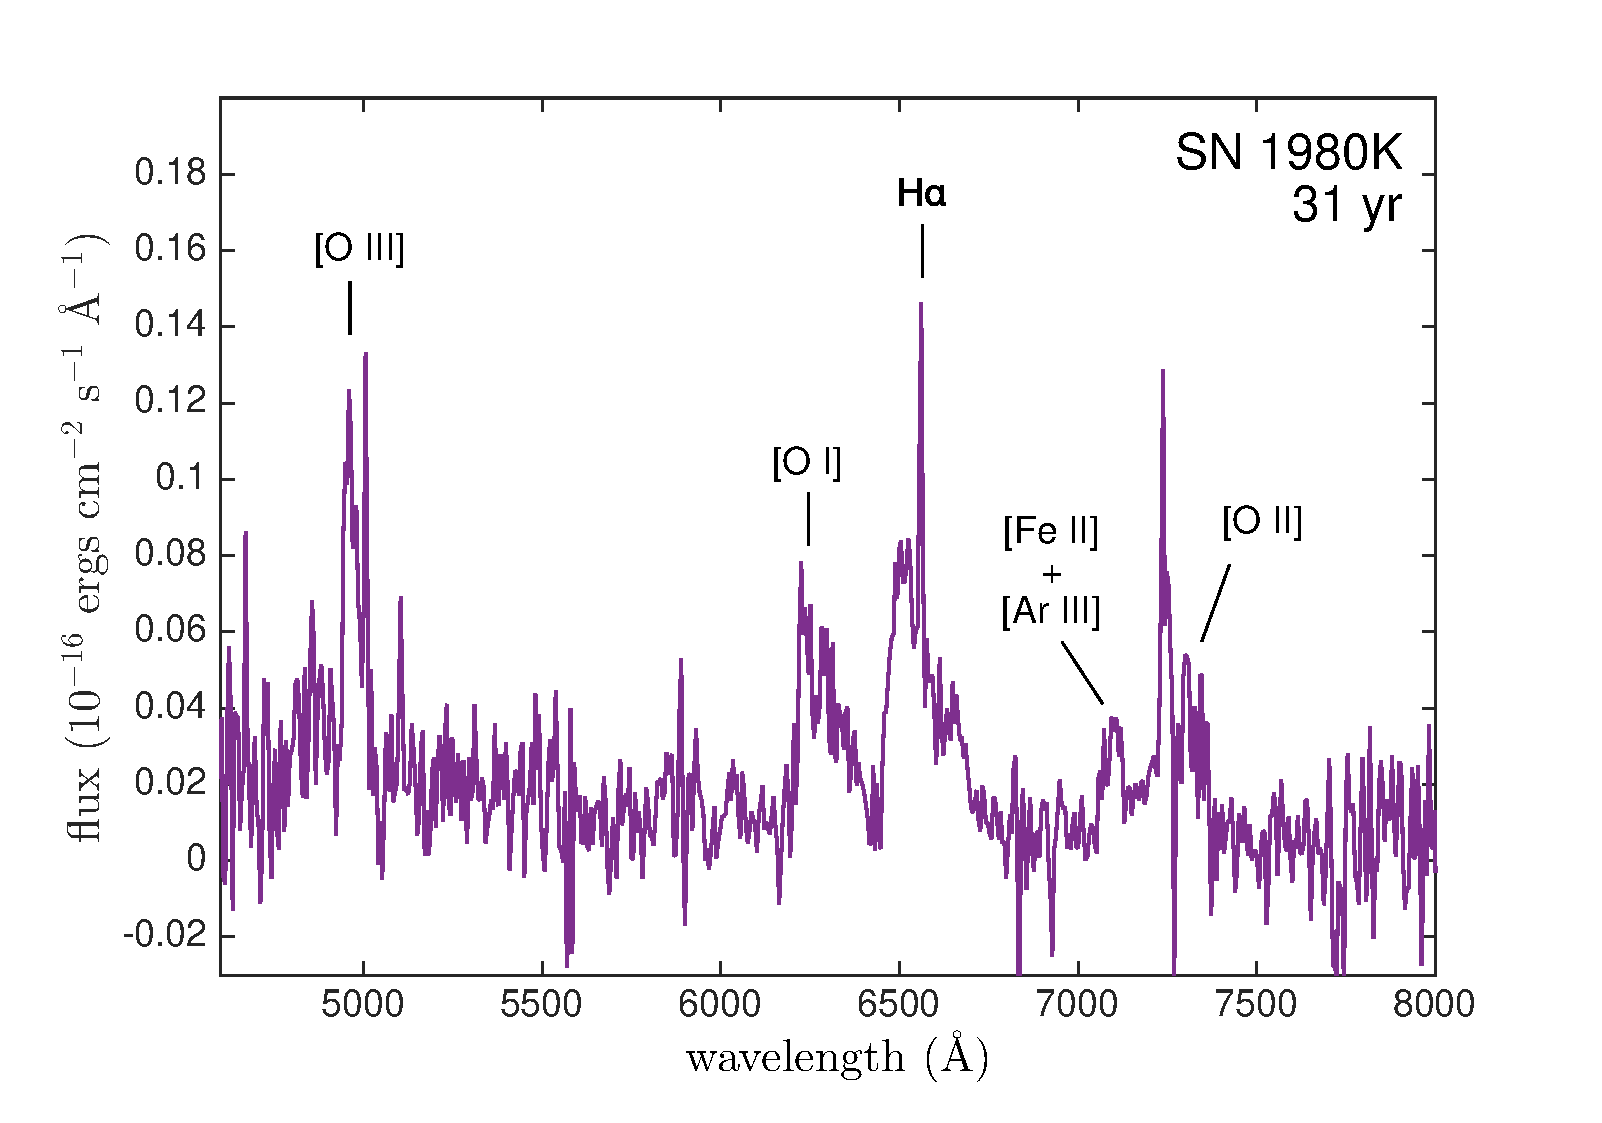
\includegraphics[clip=true,scale=0.6, trim=20 0 50 20]{chapters/chapter6/figs/80K/80K_spectrum}

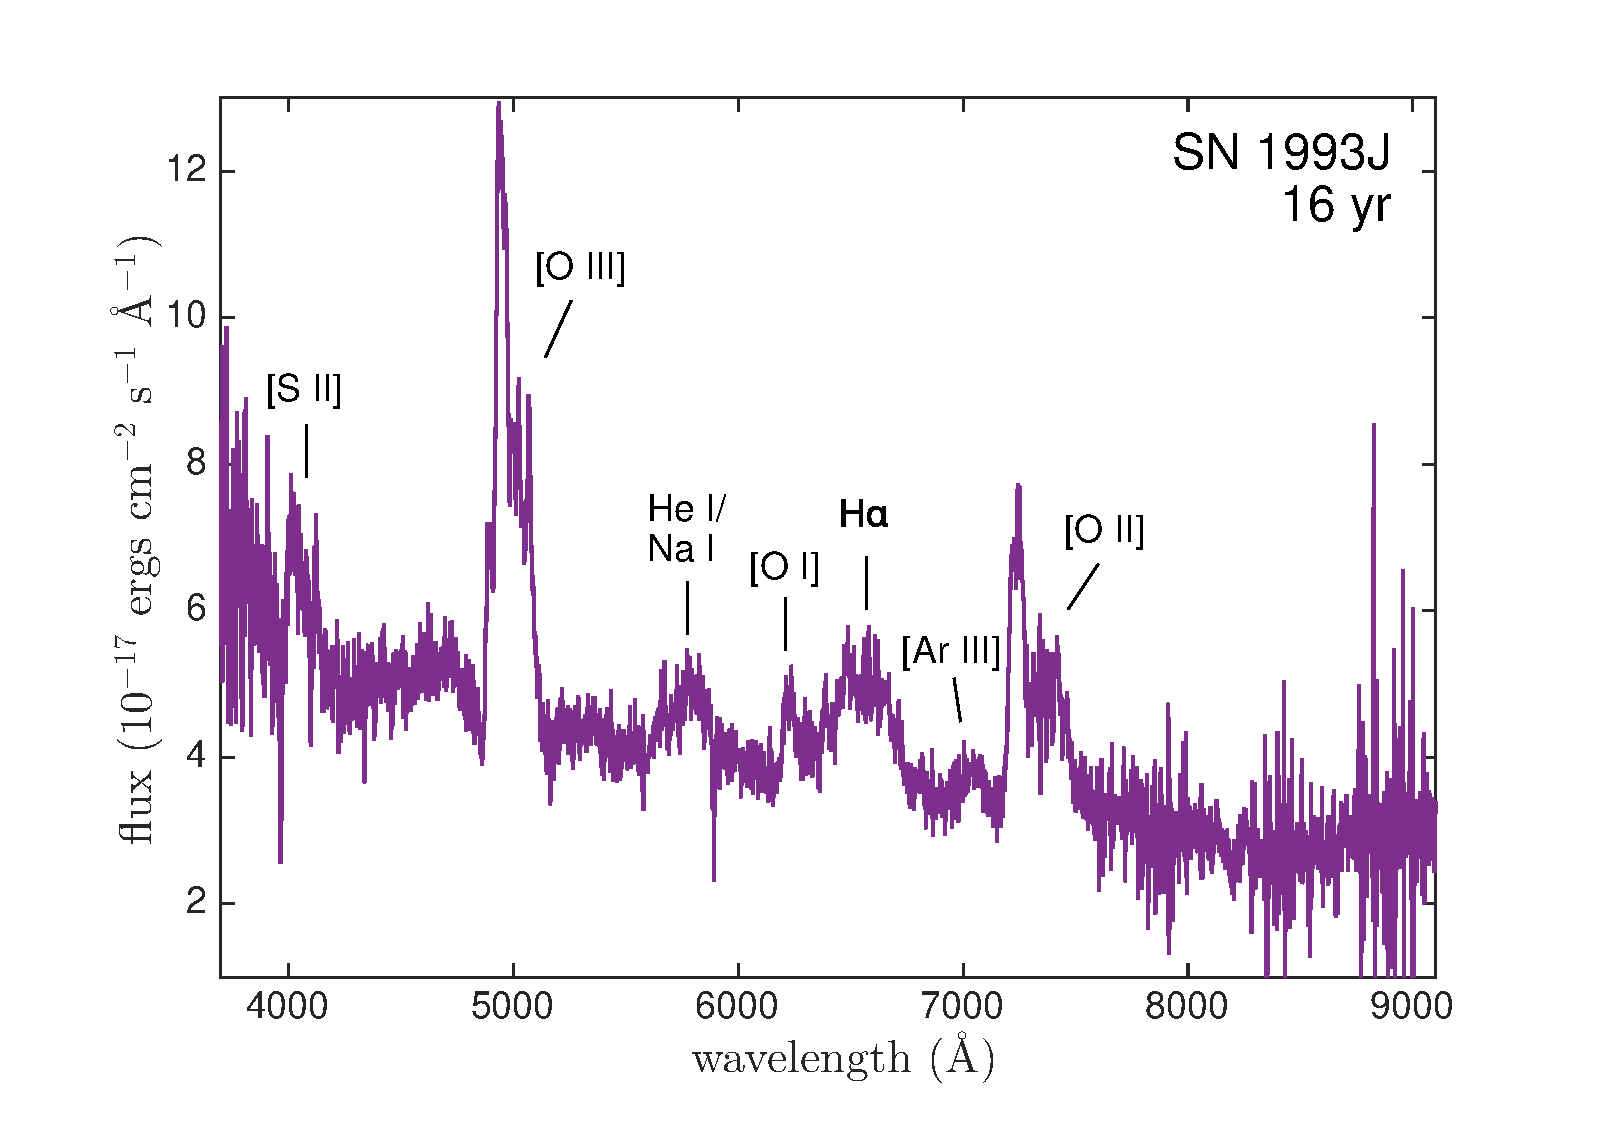
\includegraphics[clip=true,scale=0.6, trim=30 0 50 20]{chapters/chapter6/figs/93J/93J_spectrum}
\caption{{\em Above:} The optical spectrum of  SN~1980K on 9 October 2010 at 31 years post-explosion.  {\em Below:}  The optical spectrum of  SN~1993J on 9 December 2009 at 16 years post-explosion. Both spectra were originally published by \citet{Milisavljevic2012}.}
\label{spectra}
\end{figure}

\section{SN~1980K and SN~1993J}

SN~1980K is located in the Fireworks galaxy (NGC 6946) in Cygnus approximately 5.9~Mpc away \citep{Karachentsev2000}.  It was discovered by P. Wild on  28 October 1980 and  had reached a peak brightness of $V=11.4$ mag by November that year \citep{Buta1982}.   The detection of the broad H$\alpha$ line in early spectra and a linearly decaying light curve after peak brightness resulted in its classification as a Type IIL supernovae \citep{Barbon1982}.  SN~1980K continued to decline steadily in the optical although it was still detected almost seven years after maximum light by narrow passband imaging \citep{Fesen1988}.  Follow-up low dispersion observations found that the spectra exhibited broad H$\alpha$ and [O~{\sc i}]$\lambda\lambda$6300,6363~\AA\  emission with other weaker optical lines also present.  
%The SN was observed again in 2010 by \citet{Milisavljevic2012} and it is these late-time observations at 31 years after outburst that I will be interested in here.  

Spectroscopic and photometric observations of SN~1980K have revealed a very slow monotonic fading over a period of $\sim$20 years.  This unusually slow rate of decline suggested that the observations may in fact be a product of light echoes scattering off  and heating circumstellar material as discussed in Section \ref{scn:le}.  This was first suggested for SN1980K by \citet{Chevalier1986} based on early observations in the first year after outburst.  Further modelling and analyses of late-time observations performed by \citet{Sugerman2012}  found that light echoes were indeed present and that the evolution of the observations could be explained by scattered and thermal echoes off a thin circumstellar shell of dust of mass $\lesssim 0.02$~M$_{\odot}$ approximately 14--15 lightyears from the progenitor.  Of particularly relevance was their discussion of the origin of the broad, high velocity H$\alpha$ and [O~{\sc i}]$\lambda\lambda$6300,6363~\AA\ lines which were not present in the early spectra during the first two years.  They concluded that the shape of these lines could not be a product of a light echo since the high velocities seen in late-time spectra were not present in early spectra.

In 1981, the emergence of a near-IR flux excess provided the first indications of dust in the ejecta of SN~1980K \citep{Dwek1983}.  However, it could not be confirmed whether this excess IR flux was the result of newly-formed dust condensing in the ejecta or from pre-existing grains located in a circumstellar shell and illuminated by radiation from the outburst.  In addition to the detection of the signature emission from hot dust grains in the near-IR, highly blue-shifted line profiles in the optical spectra of SN~1980K have been observed for many years after\citep{Fesen1990,Fesen1994,Fesen1995,Fesen1999}.  The presence of dust in ejecta was postulated by \citet{Milisavljevic2012} based on the observed blue-shifting of the optical line profiles which are still present even in very late-time spectra (31 years). It is these late blue-shifted line profiles of SN~1980K at 31 years that I have modelled and present here.  An explosion date of 2 October 1980 \citep{Montes1998} is adopted for all models.


SN~1993J is a very well-observed and important supernova and is only surpassed  by SN~1987A in regards to the quality and frequency of its observations.  It is located in the nearby M81 galaxy 3.6~Mpc away \citep{Freedman1994} and was discovered on 28 March 1993 \citep{Ripero1993}.  It reached a maximum brightness of $V=10.8$ mag making it the brightest supernova in the northern hemisphere since SN~1954A. It was swiftly classified as a Type II supernova due to early spectra exhibiting an almost featureless blue continuum.  However, its evolution was atypical and the appearance of He lines in later spectra resulted in its classification as a Type IIb.  The similarities to Type Ib and Type Ic supernovae were noted however and this supernova has been very important for understanding the relationship between the Type I and Type II CCSN categories \citep{Fillipenko1993,Garnavich1993}.  Extensive reviews of SN~1993J are given by \citet{Wheeler1996}, who cover the early evolution of the object, and by \citet{Matheson2000a,Matheson2000b} who discuss the later evolution of the optical spectra.  

SN~1993J is relatively isolated and quite close meaning that it has proved to be an ideal candidate for regular monitoring in the X-ray, radio and optical.  I was particularly interested in late-time optical spectra obtained at 16 years post-outburst and the presence, or otherwise, of dust in the ejecta as postulated by \citet{Fransson2005} and \citet{Milisavljevic2012}.  An explosion date of 27 March 1993 \citep{Baron1993} is adopted for all models.

\subsection{The Late-Time Optical Spectra of SN~1980K and SN~1993J}

Electronic versions of the late-time spectra of both SN~1980K and SN~1993J were provided by Dr Dan Milisavljevic.  These spectra were published in \citet{Milisavljevic2012} and I present them here in Figure \ref{spectra}.

The spectra of SN 1980K were obtained on 9 October 2010 using the  2.4m Hiltner telescope at the Michigan--Dartmouth--Massachusetts Institute of Technology (MDM) observatory. The Mark III Spectrograph was used with a SITe $1024 \times 1024$ CCD detector and a $1.2'' \times 4.5'$ slit. Exposures were $2 \times 3000$~s and spectra spanned the wavelength range $4600-8000$~\AA\ with a spectral resolution of 7~\AA. The spectrum presented in Figure \ref{spectra} is of SN~1980K at approximately 31 years after outburst. Significant blue-shifting can be seen in virtually all lines, but especially in the H$\alpha$ and [O~{\sc i}]$\lambda$6300,6363~\AA\ lines which exhibit a pronounced flux bias towards the blue and a strongly blue-shifted peak (see Figure \ref{spectra}).  Narrow nebular lines of H$\alpha$ and [O~{\sc iii}] provide useful rest velocity reference points and the small recession velocity of 40~km~s$^{-1}$ of NGC~6946 has been corrected for.

The optical spectrum of SN 1993J was obtained on 9 December 2009 with the 6.5m Multiple Mirror Telescope (MMT) at Mt. Hopkins in Arizona using the HECTOSPEC optical fibre fed spectrograph. Spectra from the $1.5''$ diameter fibres covered the wavelength range of $3700-9200$~\AA\  with a full-width at half maximum (FWHM) resolution of 5~\AA.  The total exposure time was 3600~s. The observations were obtained as a part of a survey of the supernova remnants in M81.  SN~1993J was approximately 16 years old when the spectra were obtained.  Many of the lines in its optical spectrum exhibit a flux bias towards the blue and also display noticeable substructure (see Figure \ref{spectra}).  They are generally broad and  there is a significant degree of blending between lines.  The lines least blended with other lines are those of [O~{\sc iii}]$\lambda\lambda$5007,4959~\AA\ and [O~{\sc ii}]$\lambda\lambda$7319,7330~\AA\ which both demonstrate significantly asymmetrical profiles, with both the flux and the peak of their profiles shifted towards the blue.
\begin{figure}
\centering
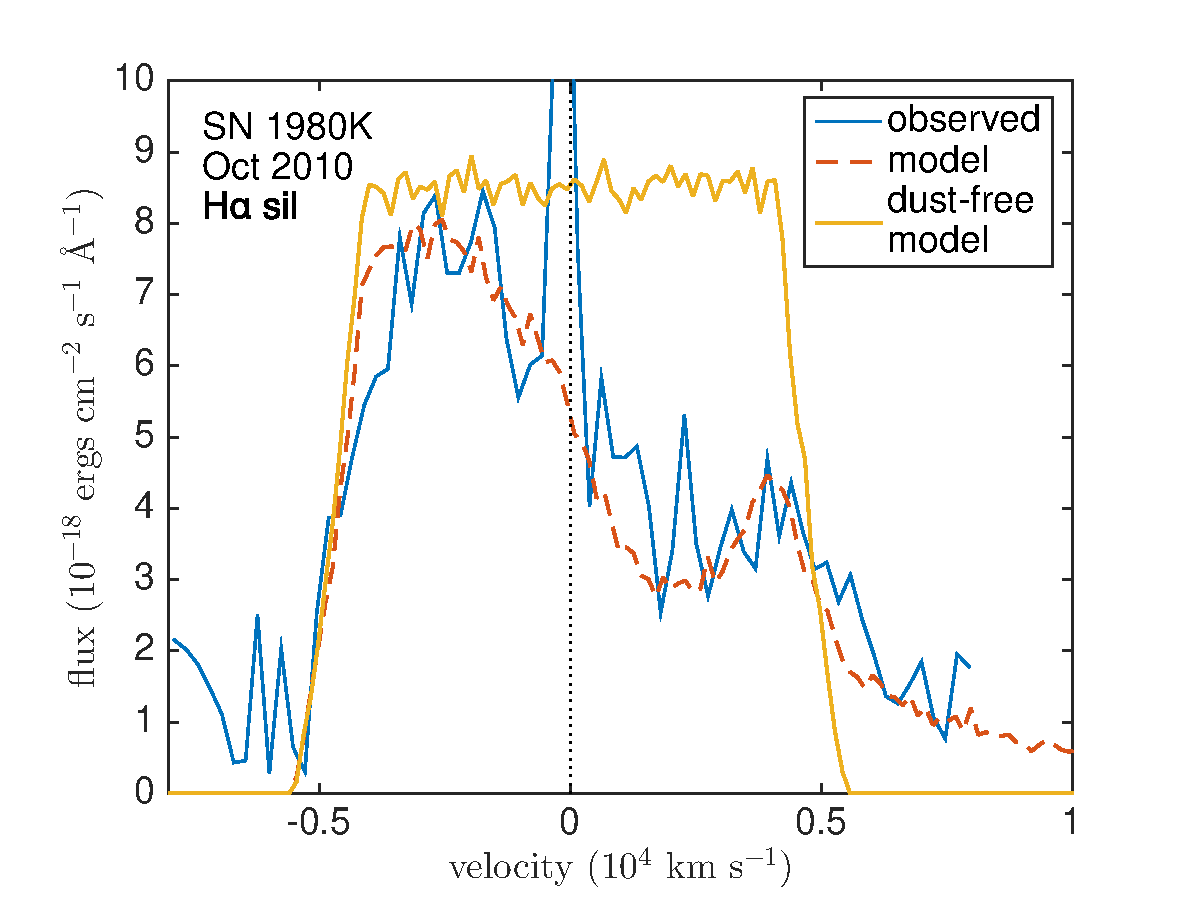
\includegraphics[clip=true,scale=0.42,trim= 20 0 50 0]{chapters/chapter6/figs/80K/smooth/Ha_with_dust_free}
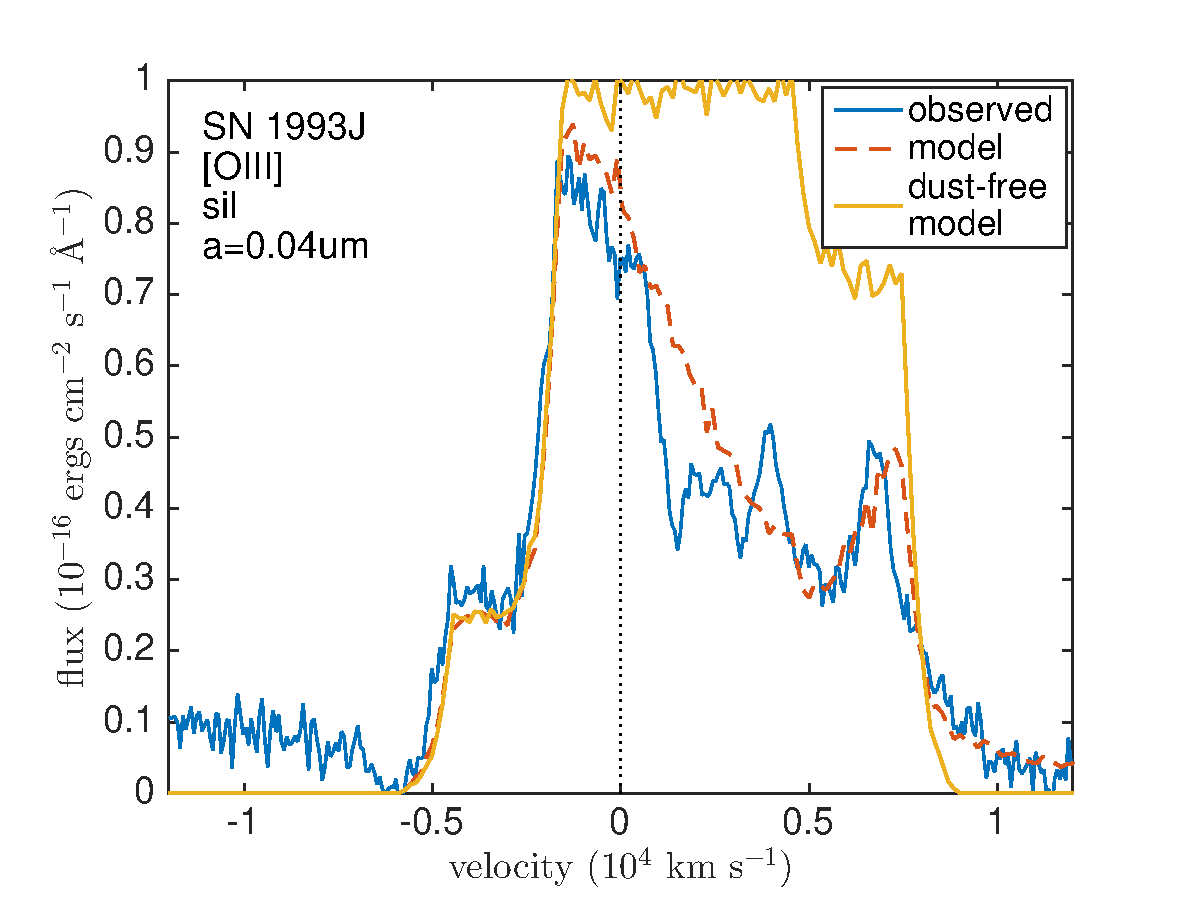
\includegraphics[clip=true,scale=0.42,trim= 17 0 50 0]{chapters/chapter6/figs/93J/smooth/OIII_with_dust_free}
\caption{Best-fitting smooth dust models along with the intrinsic dust-free boxy profile for the H$\alpha$ line profile for SN~1980K {\em (left)} and the [O~{\sc iii}]$\lambda\lambda$5007,4959~\AA\ line profile for SN~1993J {\em (right)}.  The intrinsic dust-free modelled line profile is given in yellow, the dust-affected modelled line profile in red and the observed line profile in blue.}
\label{boxy}
\end{figure}

\citet{Milisavljevic2012} reduced and calibrated the spectra of both objects by employing
standard techniques in IRAF and their own routines, removing any cosmic rays and obvious defects. The spectra have been corrected for a recession velocity of $-140$~km~s$^{-1}$ \citep{Matheson2000b}.  For further details on the observations and calibrations of these spectra, please refer to \citet{Milisavljevic2012}. 




\section{Line Profile Models of SN~1980K and SN~1993J}
\label{80K_93J_models}
My modelling of SN~1980K focussed on the H$\alpha$ line and the [O~{\sc i}]$\lambda\lambda$6300,6363~\AA\  doublet.  Both of these line profiles exhibited a very strong blue-shifted asymmetry indicative of the presence of dust in the ejecta and, like SN~1987A, were sufficiently distinct that they provided the best options for modelling purposes.  Other lines were either too blended with each other or too noisy to be reliable.  

SN~1993J exhibited its strongest line asymmetries in the oxygen lines, and in particular I focussed my modelling on the [O~{\sc ii}]$\lambda\lambda$7319,7330~\AA\  and [O~{\sc iii}]$\lambda\lambda$5007,4959~\AA\  doublets mentioned above.  The [O~{\sc i}]$\lambda\lambda$6300,6363~\AA\ doublet was not modelled for SN~1993J as it was quite blended with the H$\alpha$ line and the two lines could not be easily extricated.  The [O {\sc ii}] and [O {\sc iii}] lines being more distinct were therefore the more sensible candidates for modelling.

\afterpage{
\begin{landscape}
\centering
\setlength{\tabcolsep}{4pt}
\begin{table}
\centering
%	\begin{minipage}{180mm}
	\caption{The parameters used for the smooth and clumped models of SN~1980K for media composed of 100\% amorphous carbon dust grains of radius $3.5$~$\mu$m, or 100\% silicate dust grains of radius $0.1$~$\mu$m.  Optical depths are given from $R_{in}$ to $R_{out}$ at $\lambda = 6300$~\AA\  for [O~{\sc i}] and $\lambda = 6563$~\AA\  for H$\alpha$.  The doublet ratio for the [O~{\sc i}]$\lambda\lambda$6300,6363~\AA\  was fixed to be 3.1.  Smooth dust models are listed in the first four rows and clumped dust models in the last four rows.}
	\label{80K}
	\centering
  	\begin{tabular}{@{} ccccccccccccccc @{}}
    	\hline
  & clumped? & species &$a$&$V_{max}$ & $V_{min}$ & $R_{in}/R_{out}$ & $\beta$ &  $R_{out}$ & $R_{in}$ & doublet & $\tau_{\lambda}$  & $f$ & $R_{clump}$ &$M_{dust}$ \\
	&& &($\mu$m)&(km~s$^{-1}) $& (km~s$^{-1} $)& &&  (10$^{17}$cm) & (10$^{17}$cm) &ratio&&&(10$^{17}$cm) &($M_{\odot}$)  \\
	\hline
	H$\alpha$  &no&sil & 5500 & 4125 & 0.75  & 2.0 & 0.1 & 5.2 & 3.9 & - & 1.41 & - & - &0.1\\ \relax
H$\alpha$  &no&amC& 3.5&5500 & 4125 & 0.75  & 2.0  & 5.2 & 3.9 & - & 0.57 & - &  -& 0.3\\ \relax
[O~{\sc i}]  &no&sil&0.1& 5500 & 4125 & 0.75  & 4.0  & 5.2 & 3.9 & 3.1 & 2.81 & - & - & 0.2\\ \relax
[O~{\sc i}]  &no&amC&3.5& 5500 & 4125 & 0.75  & 4.0  & 5.2 & 3.9 & 3.1 & 1.24  & - & -& 0.65\\
\\
H$\alpha$  &yes&sil & 0.1&5500 & 4125 & 0.75  & 2.0  & 5.2 & 3.9 & - & 1.68 & 0.1 & 0.2 & 0.12\\ \relax
H$\alpha$  &yes&amC& 3.5&5500 & 4125 & 0.75  & 2.0  & 5.2 & 3.9 & - & 0.73 & 0.1 &  0.2& 0.38\\ \relax
[O~{\sc i}]  &yes&sil&0.1& 5500 & 4125 & 0.75  & 4.0  & 5.2 & 3.9 & 3.1 & 2.81 & 0.1 & 0.2 & 0.3\\ \relax
[O~{\sc i}]  &yes&amC&3.5& 5500 & 4125 & 0.75  & 4.0  & 5.2 & 3.9 & 3.1 & 1.72  & 0.1 & 0.2& 0.9\\
    \hline
  \end{tabular}
%\end{minipage}
\end{table}
\end{landscape}
\begin{figure}[!t]
\centering
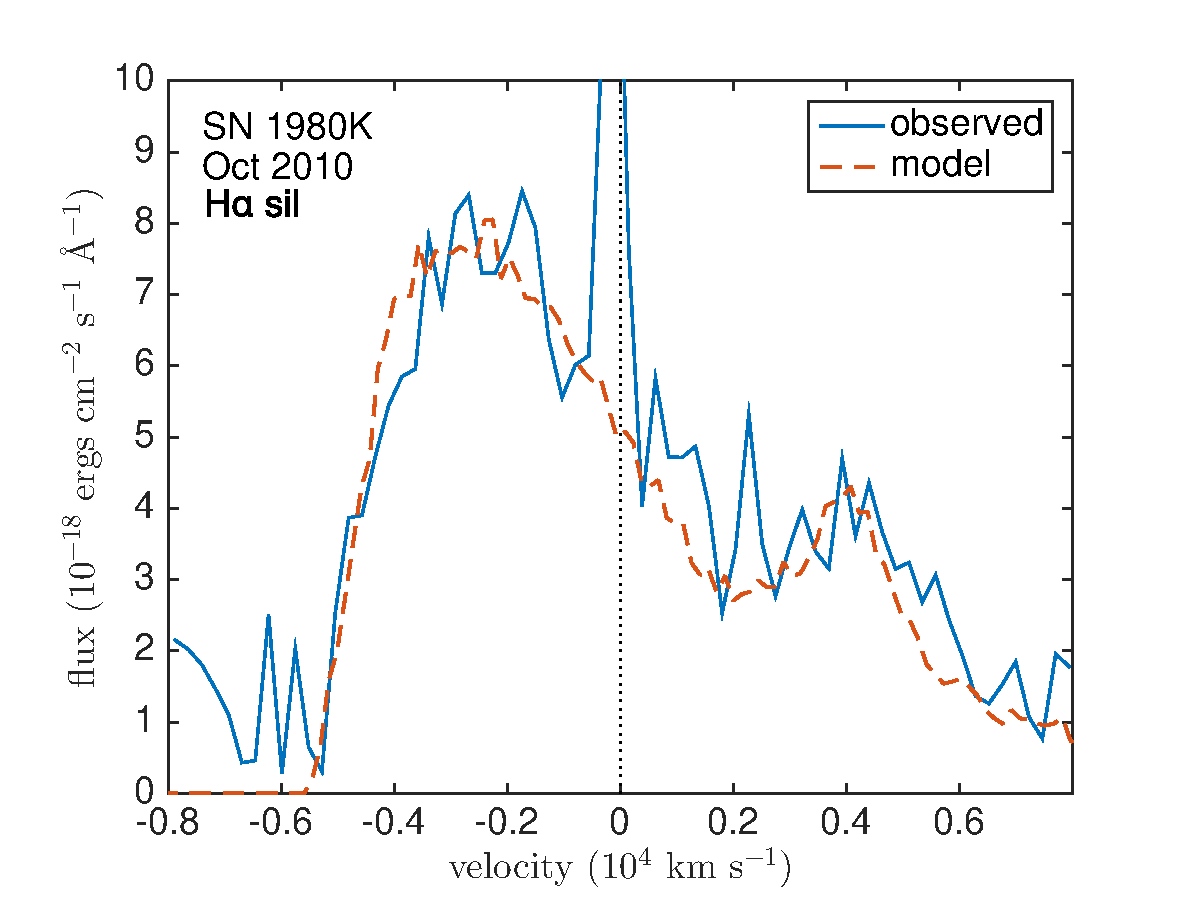
\includegraphics[scale=0.4,clip=true, trim=20 0 40 20]{chapters/chapter6/figs/80K/smooth/Ha}
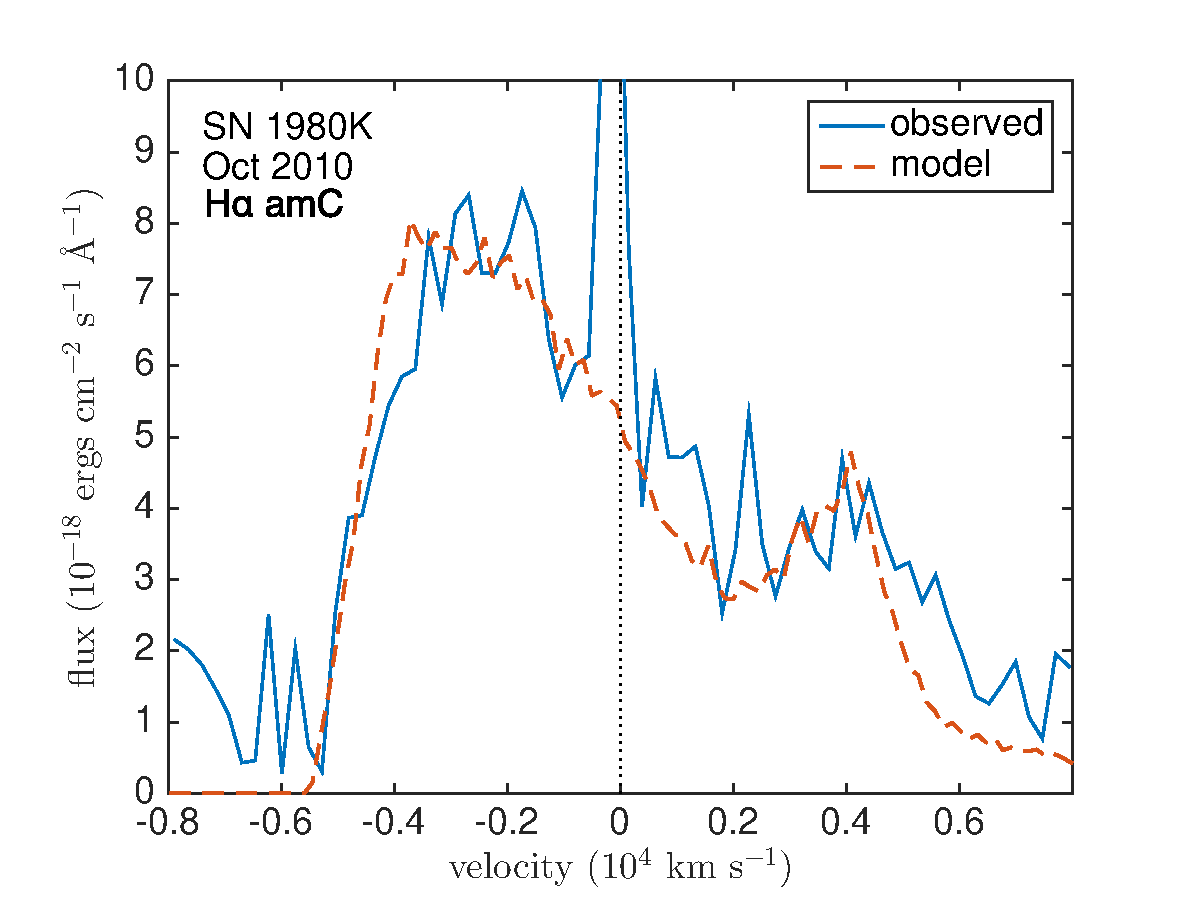
\includegraphics[scale=0.4,clip=true, trim=20 0 40 20]{chapters/chapter6/figs/80K/smooth/Ha_amC}

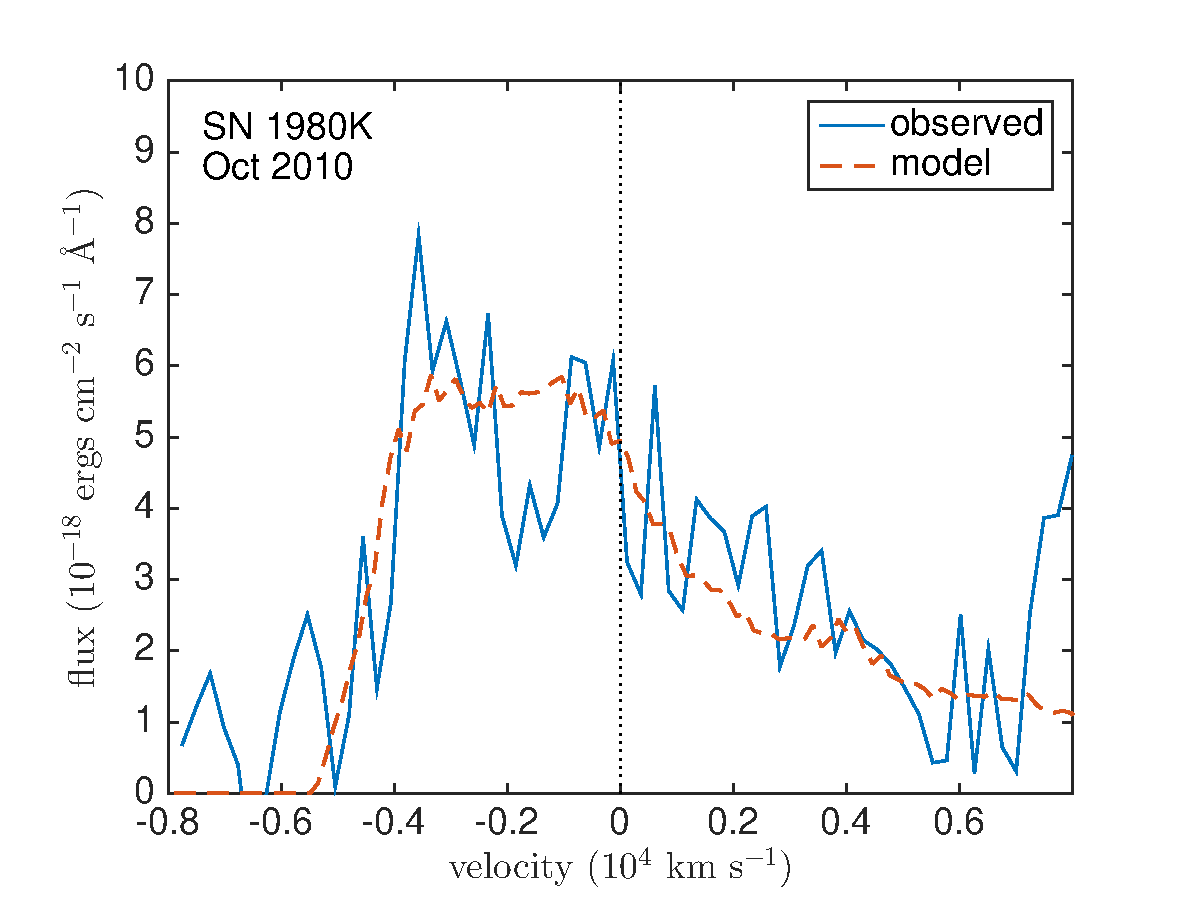
\includegraphics[scale=0.4,clip=true, trim=20 0 40 20]{chapters/chapter6/figs/80K/smooth/OI}
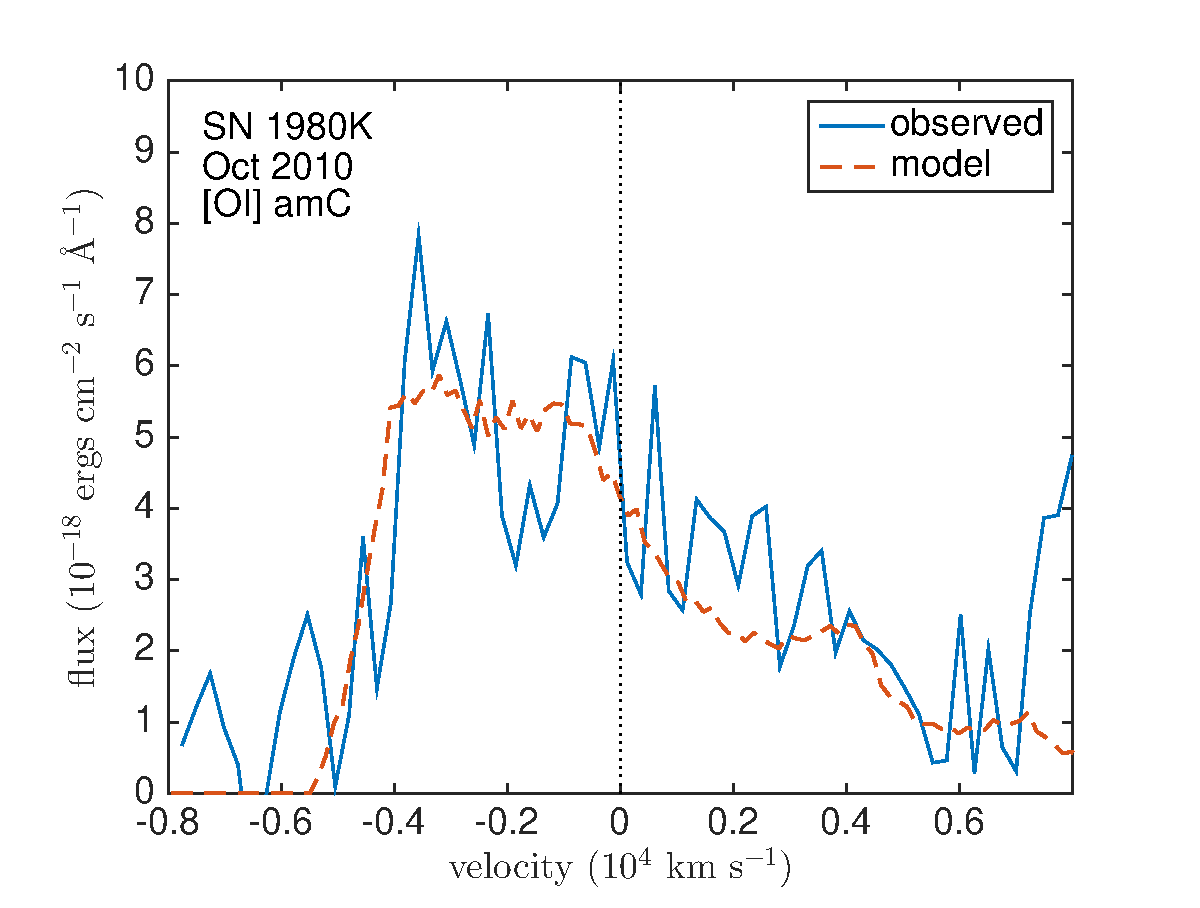
\includegraphics[scale=0.4,clip=true, trim=20 0 40 20]{chapters/chapter6/figs/80K/smooth/OI_amC}
\caption{Best smooth dust fits to the SN~1980K H$\alpha$ line ({\em top})  and the  [O~{\sc i}]$\lambda\lambda$6360,6363~\AA\ doublet ({\em bottom}) for the parameters detailed in Table \ref{80K}.  Smooth dust fits with astronomical silicate grains of radius $a=0.1$~$\mu$m are presented on the left and smooth dust fits with amorphous carbon grains of radius $a=3.5$~$\mu$m are presented on the right.  For the [O~{\sc i}] doublet, zero velocity was set at $\lambda=6300$~\AA.}
\label{80K_smooth}
\end{figure}

}


My approach to modelling the line profiles of both SN~1980K and SN~1993J followed the same principles as for SN~1987A that I detailed in Section \ref{results}.  I began the modelling by considering a smooth, coupled distribution of dust and gas before moving on to consider the effect on these models of including a clumped dust geometry whilst maintaining a smooth emissivity distribution.  I first examined the line profiles in order to determine the maximum and minimum velocities before moving on to establish approximately the exponent of the dust and gas density distributions.  Having fixed the starting values for these quantities, I iterated over the grain size and dust mass in order to fit the profile.  I also occasionally  varied the other parameters in order to optimise the fits to the data. I assumed that the oxygen doublets were optically thin for both SN~1980K and SN~1993J and therefore adopted a constant intrinsic flux ratio of 3.1 between the [O~{\sc i}]$\lambda\lambda$6300,6363~\AA\  components, 1.2 between the [O~{\sc ii}]$\lambda\lambda$7319,7330~\AA\  components and 2.98 between the [O~{\sc iii}]$\lambda\lambda$5007,4959~\AA\  components according to the theoretical flux ratios as detailed by \citet{Zeippen1987} and \citet{Storey2000}.  The intrinsic line profiles before dust effects for SN~1980K and SN~1993J both needed to be very `boxy', that is, the ratio of the inner to outer radii was very high so that the overall profile has a very square shape (see Figure \ref{boxy}).  I present the intrinsic dust-free profile along with the best-fitting smooth H$\alpha$ model for SN~1980K in the left pane of Figure \ref{boxy} and the intrinsic dust-free profile for the best-fitting smooth [O~{\sc iii}]$\lambda\lambda$5007,4959~\AA\ model for SN~1993J in the right pane of Figure \ref{boxy}.

\begin{figure}[!t]
\centering
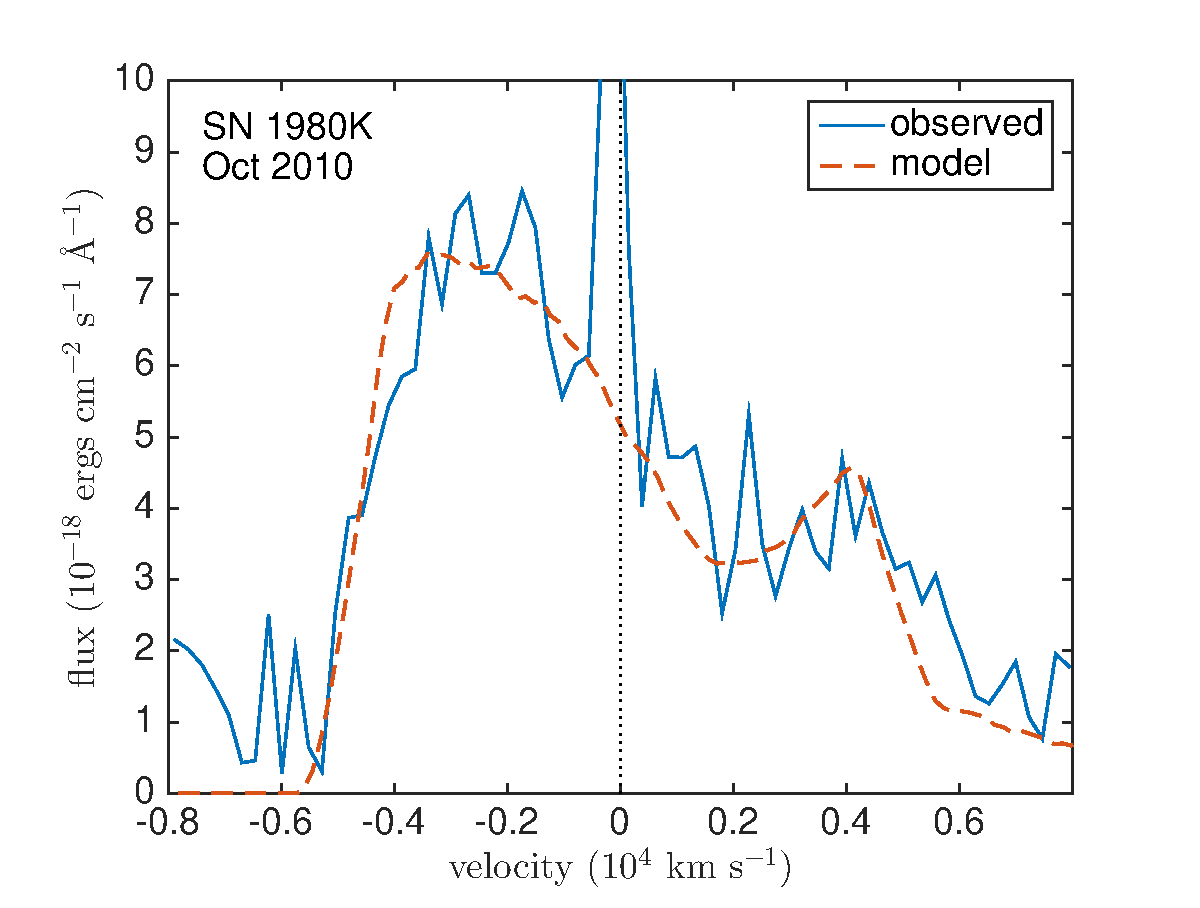
\includegraphics[scale=0.4,clip=true, trim=20 0 40 20]{chapters/chapter6/figs/80K/clumped/Ha}
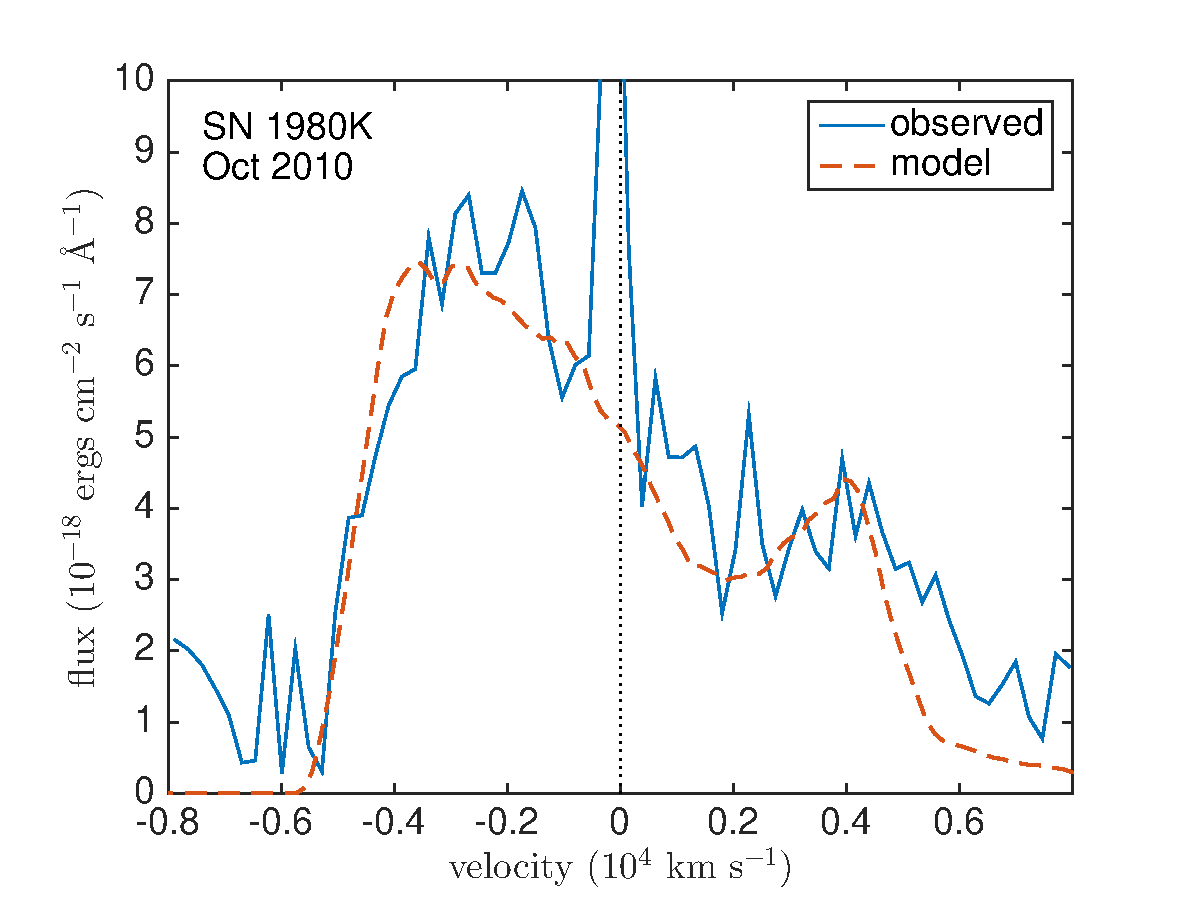
\includegraphics[scale=0.4,clip=true, trim=20 0 40 20]{chapters/chapter6/figs/80K/clumped/Ha_amC}

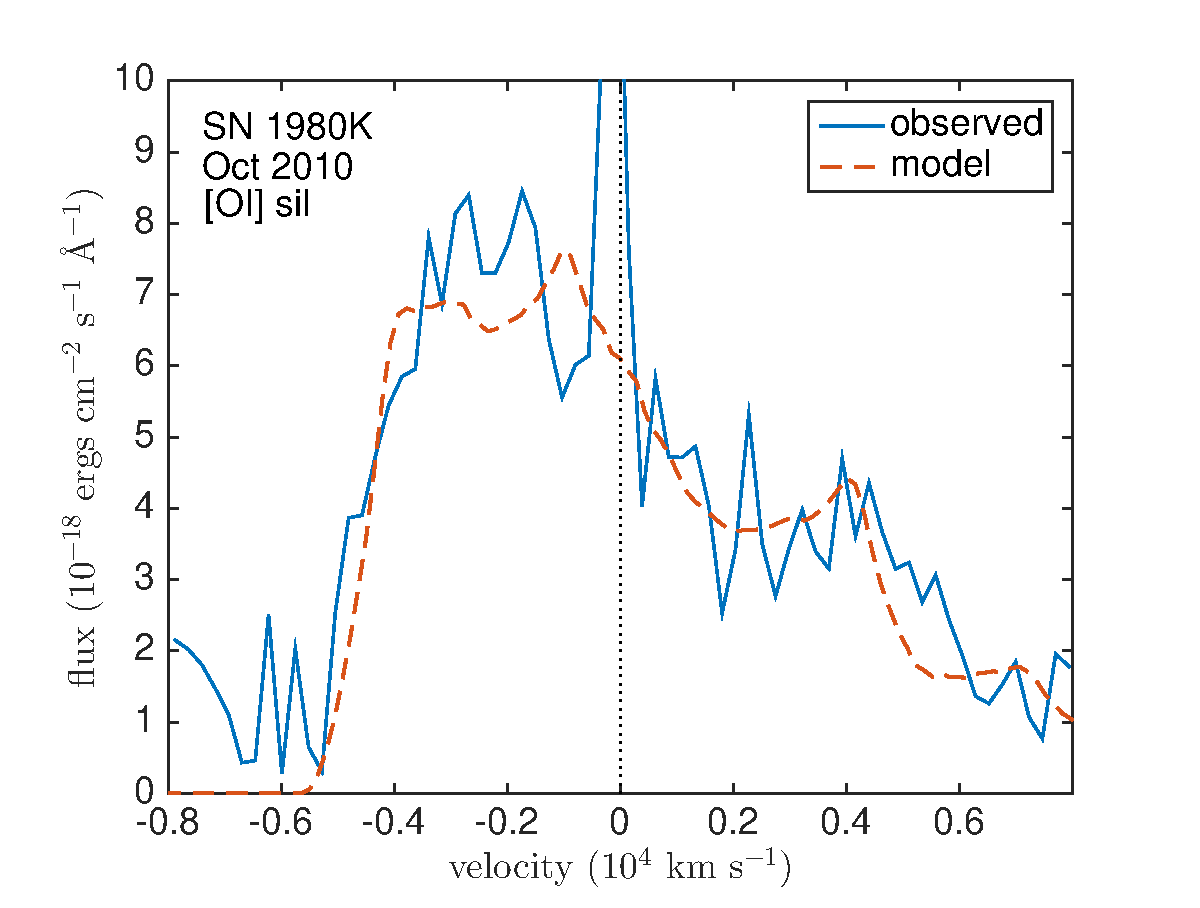
\includegraphics[scale=0.4,clip=true, trim=20 0 40 20]{chapters/chapter6/figs/80K/clumped/OI}
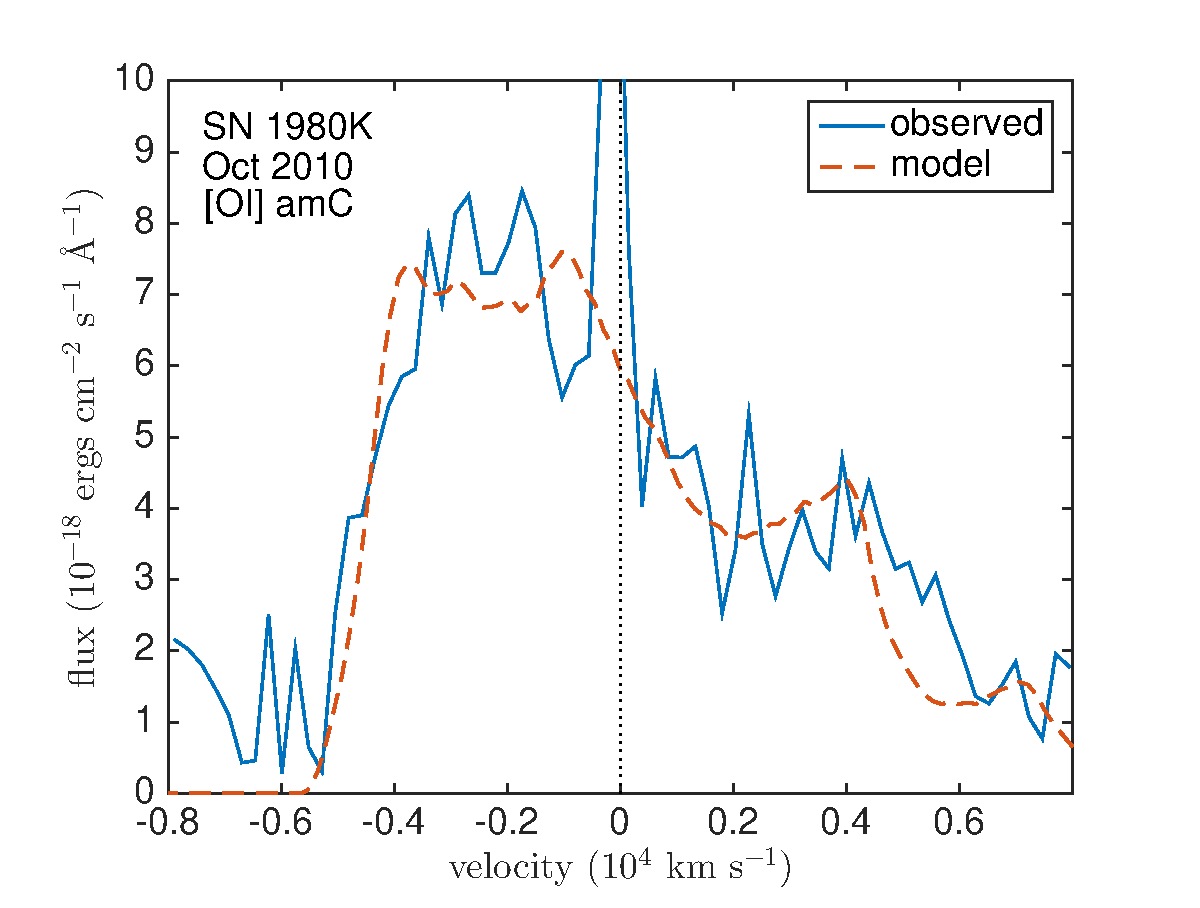
\includegraphics[scale=0.4,clip=true, trim=20 0 40 20]{chapters/chapter6/figs/80K/clumped/OI_amC}
\caption{Best clumped dust fits to the SN~1980K H$\alpha$ line ({\em top}) and the [O~{\sc i}]$\lambda\lambda$6360,6363~\AA\ doublet ({\em bottom}) for the parameters detailed in Table \ref{80K}.  Clumped dust fits with astronomical silicate grains of radius $a=0.1$~$\mu$m are presented on the left and clumped dust fits with amorphous carbon grains of radius $a=3.5$~$\mu$m are presented on the right. For the [O~{\sc i}] doublet, zero velocity was set at $\lambda=6300$~\AA.}
\label{80K_clumped}
\end{figure}

The parameters for the smooth and clumped dust fits  that I obtained for SN~1980K and SN~1993J are detailed in Tables \ref{80K} and \ref{93J} respectively. The smooth dust line profile fits for SN~1980K are presented in Figure \ref{80K_smooth} and the clumped dust line profile fits are presented in Figure \ref{80K_clumped}.  The smooth dust line profile fits for SN~1993J are presented in Figure \ref{93J_smooth} and the clumped dust line profile fits are presented in Figure \ref{93J_clumped}.  

\subsection{SN~1980K Dust Smooth Models}

I obtained good fits to both the H$\alpha$ line and the [O~{\sc i}]$\lambda\lambda$6300,6363~\AA\  doublet from SN~1980K (see Figure \ref{80K_smooth}).  In particular, an extended wing on the red side of the profile was seen in both cases. This was more important for the H$\alpha$ line since I could be sure that it was not a product of blending with an adjacent broad line (the presence of an extended red wing in the [O~{\sc i}] doublet may be due to blending with the blue wing of the H$\alpha$ line).  The H$\alpha$ red wing allowed me to place constraints on the albedo.  A high albedo of $\omega\approx0.8$  was required to reproduce the flux in the region between $+6000$ and $+8000$~km~s$^{-1}$.  Astronomical silicate grains \citep{Draine1984} of radius $a=0.1$~$\mu$m have an albedo of this magnitude at this wavelength, but amorphous carbon grain are never this glassy regardless of their size.  As well as the best-fitting silicates model in Figure \ref{80K_smooth}, I include line profile fits using a large grain size ($a=3.5$~$\mu$m) for amorphous carbon to generate as high an albedo as possible ($\omega\approx0.6$) illustrating the slightly worse, although still reasonably good, fit to the H$\alpha$ line.  

\subsection{SN~1980K Dust Clumped Models}

Motivated by the modelling of SN~1987A, I adopted a clumped dust structure with a clump volume filling factor of $f=0.1$ with clumps of width $R_{clump}=R_{out}/25$.  All dust was located in clumps but the gas emission remained distributed smoothly according to the distribution derived for the smooth models.  A summary of the parameters for the best-fitting clumped models is presented in Table \ref{80K} and the fits are presented in Figure \ref{80K_clumped}.

\subsection{SN~1980K Discussion}
\label{scn:discuss}
 
The models for the H$\alpha$ and [O~{\sc i}]$\lambda\lambda$6300,6363~\AA\ profiles are broadly consistent with each other.  The primary differences in the derived parameters are in the exponents of the density distributions and the total dust masses, with the oxygen distribution following a steeper density trend than the more diffusely emitted hydrogen.  In a similar manner to the early phase models of SN~1987A, the [O~{\sc i}]$\lambda\lambda$6300,6363~\AA\ line profile models require significantly greater dust masses than the H$\alpha$ models. I believe that this is likely to be due to the same reason that I discuss in Section \ref{complex}, namely that the dust forming regions are likely to be concentrated towards those zones which are oxygen rich \citep{Kozma1998a}.  As a result, it seems possible that if the oxygen is  located in clumps along with the dust then the discrepancy in the dust masses could potentially be resolved by considering more complex, decoupled distributions of dust and gas with diffuse hydrogen emission and clumped oxygen emission.  I illustrated this possibility for SN~1987A in Chapter \ref{chp:chp5}.  I note that for the clumped models for SN~1980K and SN~1993J the difference between the dust masses derived from the [O~{\sc i}]$\lambda\lambda$6300,6363~\AA\ fits and H$\alpha$ fits is around a factor of approximately two, very similar to that seen for SN~1987A.  

 The H$\alpha$ and [O~{\sc i}] line profiles of SN~1908K both exhibit an extended scattering wing which requires a glassy dust composition with a high albedo to fit it.  Amorphous carbon models do not fit the red side of the H$\alpha$ profile very well, even for very large grain sizes. I therefore adopt a silicate dust composition, which fits the profiles somewhat better.  I note that a combination of grain species would also be capable of producing the high albedo that is required but would be expected to result in dust masses somewhere in between those of the amorphous carbon and silicate models.  The relatively low signal-to-noise ratio of both profiles means that a small degree of variation in the parameters is found to  generate modelled line profiles that also fit the data reasonably.  This is most important in the determination of the high albedo which is  based on a relatively small section of the observed line profile in the red wing of the data.  Further observations with a higher signal-to-noise ratio would be beneficial for the purposes of line profile modelling. 

\afterpage{
\begin{landscape}
\centering
\setlength{\tabcolsep}{4pt}
\begin{table}
\centering
%	\begin{minipage}{180mm}
	\caption{The parameters used for the smooth and clumped models of SN~1993J for media composed of 100\% amorphous carbon dust grains of radius $3.5$~$\mu$m, or 100\% silicate dust grains of radius $0.1$~$\mu$m.  Optical depths are given from $R_{in}$ to $R_{out}$ at $\lambda = 7319$~\AA\  for [O~{\sc ii}] and $\lambda = 4959$~\AA\  for [O~{\sc iii}].  Smooth dust models are listed in the first four rows and clumped dust models in the last four rows.}
	\label{93J}
	\centering
  	\begin{tabular}{@{} ccccccccccccccc @{}}
    	\hline
  & clumped? & species &$a$&$V_{max}$ & $V_{min}$ & $R_{in}/R_{out}$ & $\beta$  & $R_{out}$ & $R_{in}$ & doublet  & $\tau_{\lambda}$  & $f$ & $R_{clump}$& $M_{dust}$ \\
	&& &($\mu$m)&(km~s$^{-1}) $& (km~s$^{-1} $)& & & (10$^{17}$cm) & (10$^{17}$cm) &ratio&&&(10$^{17}$cm) & ($M_{\odot}$) \\
	\hline
	{[O~{\sc iii}]}  &no&sil & 0.04&6000 & 4500 & 0.75  & 7  & 3.2 & 2.4 & 2.98 & 0.65 & - & - & 0.1\\ \relax
{[O~{\sc iii}]}  &no&amC&0.2& 6000 & 4500 & 0.75  & 7  & 3.2 & 2.4 & 2.98& 0.63 & - &  -& 0.005\\ \relax
{[O~{\sc ii}]}  &no&sil& 0.1&6000 & 4500 & 0.75  & 7  & 3.2 & 2.4 & 1.23 & 0.74 & - & - & 0.05\\ \relax
{{[O~{\sc ii}]}}  &no&amC&3.5& 6000 & 4500 & 0.75  & 7 & 3.2 & 2.4 & 1.23 & 0.60  & - & - & 0.12\\
\\
{[O~{\sc iii}]}  &yes&sil &0.04& 6000 & 4500 & 0.75  & 7  & 3.2 & 2.4 & 2.98 &1.00  & 0.1 & 0.13& 0.15 \\ \relax
{[O~{\sc iii}]}  &yes&amC&0.2& 6000 & 4500 & 0.75  & 7 & 3.2 & 2.4 & 2.98 &0.96  & 0.1 &  0.13&  0.008\\ \relax
{[O~{\sc ii}]}  &yes&sil&0.1 &6000 & 4500 & 0.75  & 7   & 3.2 & 2.4 & 1.23 & 1.12 & 0.1 & 0.13 &0.08\\ \relax
{[O~{\sc ii}]}  &yes&amC& 3.5& 6000 & 4500 & 0.75  & 7& 3.2 & 2.4 & 1.23 & 0.95  & 0.1 & 0.13 &  0.18 \\ 
    \hline
  \end{tabular}

%\end{minipage}
\end{table}
\end{landscape}

\begin{figure}[!t]
\centering
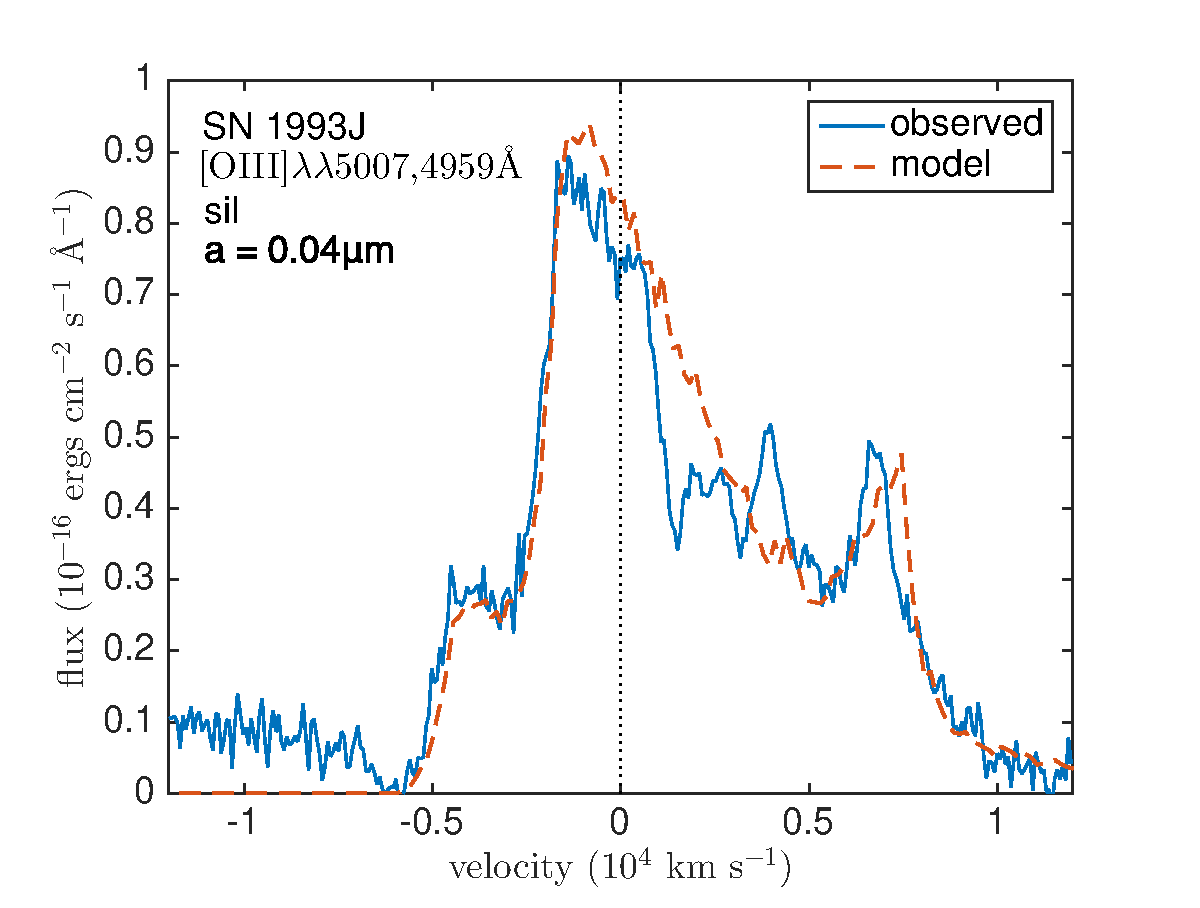
\includegraphics[scale=0.4,clip=true, trim=0 0 40 20]{chapters/chapter6/figs/93J/smooth/OIII} \hspace{0.5mm}
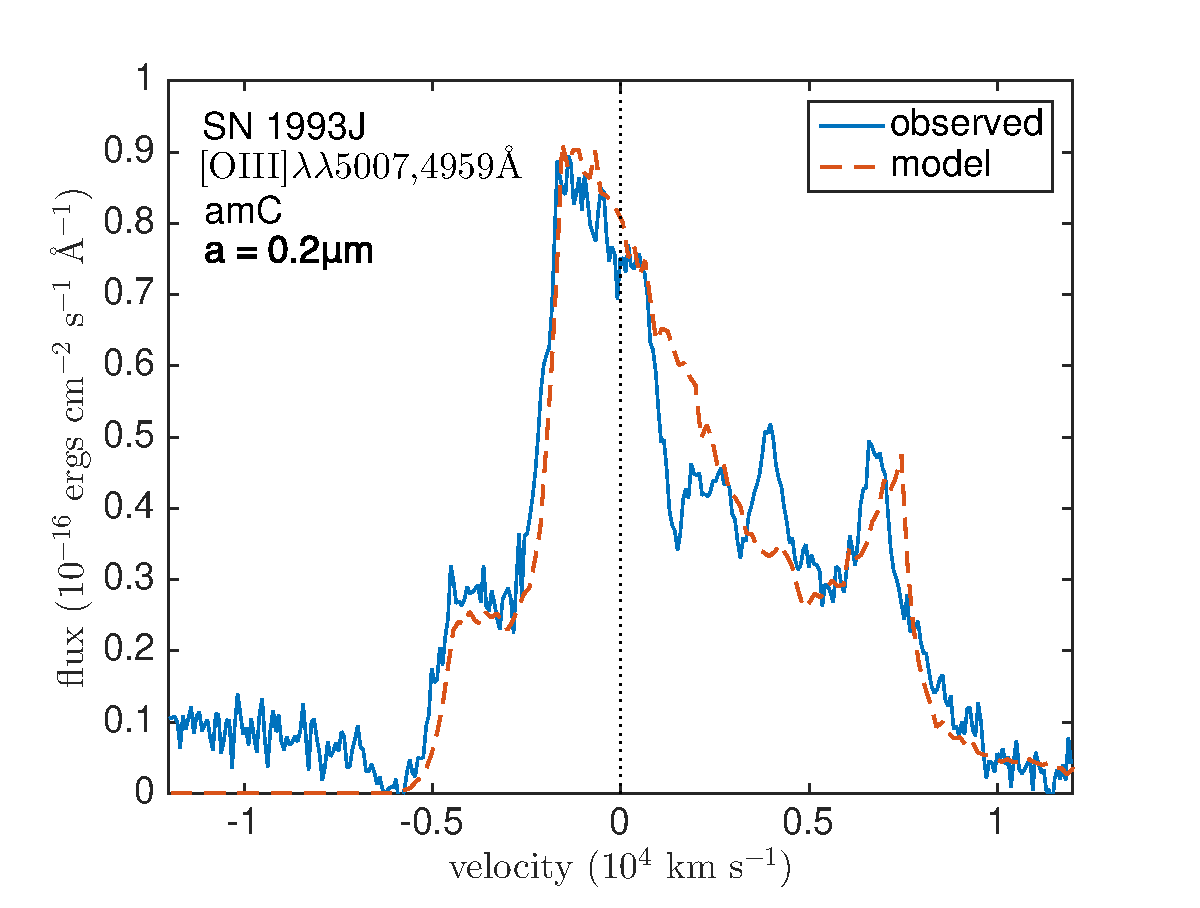
\includegraphics[scale=0.4,clip=true, trim=40 0 40 20]{chapters/chapter6/figs/93J/smooth/OIII_amC}

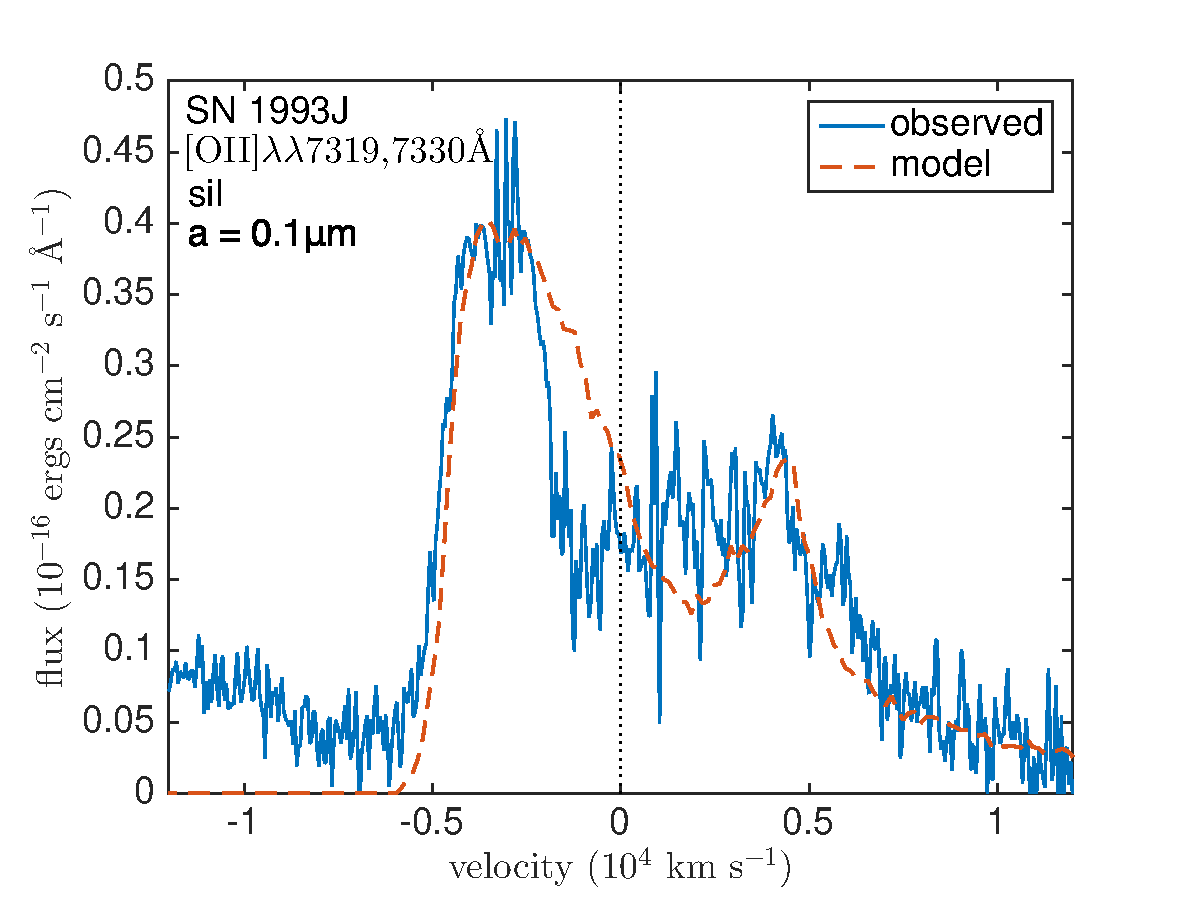
\includegraphics[scale=0.4,clip=true, trim=0 0 40 20]{chapters/chapter6/figs/93J/smooth/OII}
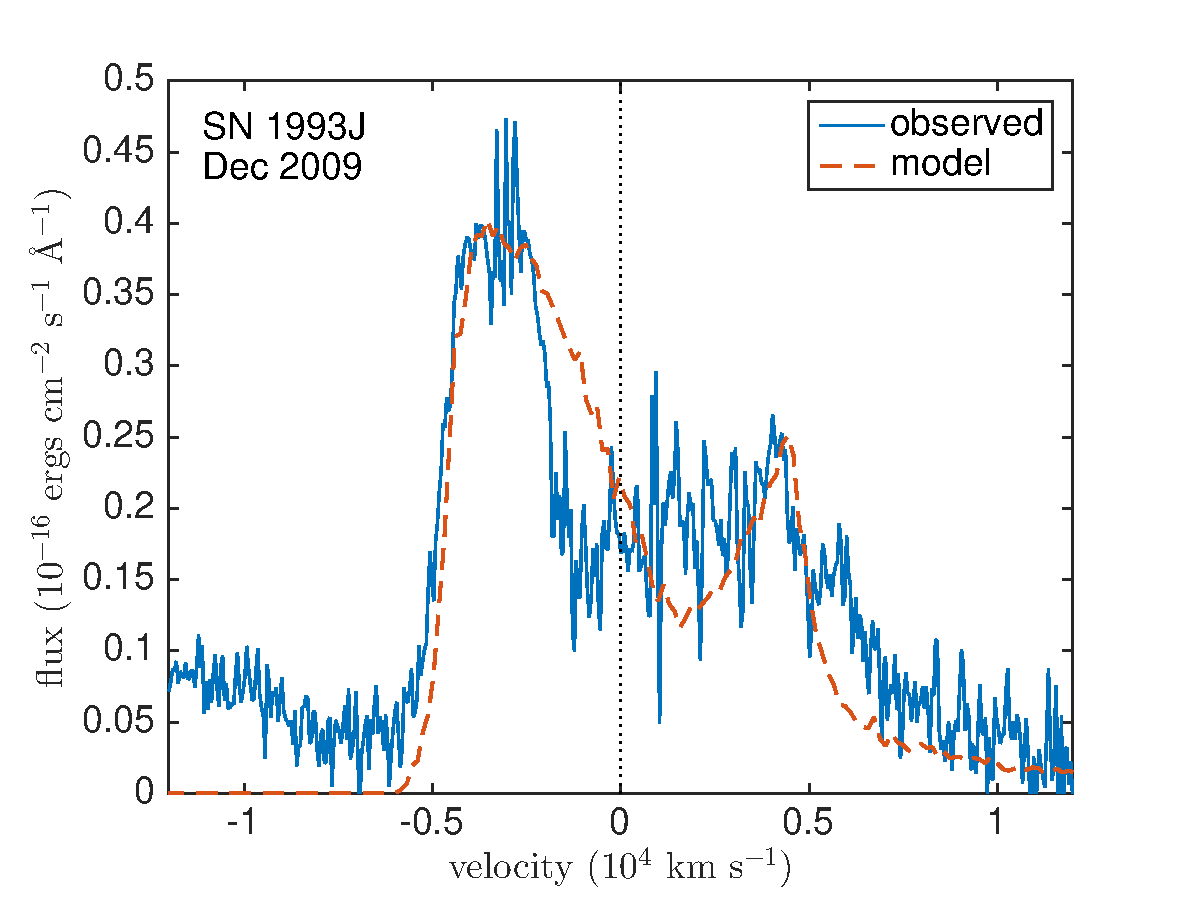
\includegraphics[scale=0.4,clip=true, trim=30 0 40 20]{chapters/chapter6/figs/93J/smooth/OII_amC}
\caption{Best smooth dust fits to the SN~1993J [O~{\sc iii}]$\lambda\lambda$5007,4959~\AA\ doublet ({\em top}) and the [O~{\sc ii}]$\lambda\lambda$7319,7330~\AA\ doublet ({\em bottom}) for the parameters detailed in Table \ref{93J}.  For the [O~{\sc ii}] doublet, zero velocity was set at $\lambda=7319$~\AA\ and for the [O~{\sc iii}] doublet, zero velocity was set at $\lambda=4959$~\AA.  Compositions and sizes are as detailed on the plots.}
\label{93J_smooth}
\end{figure}
}

There has been limited discussion of the dust mass that could be present in the ejecta of SN~1980K other than its predicted existence based on its asymmetrical optical line profiles.  The first suggestion of dust in the ejecta of SN~1980K was based on a near-IR flux excess seen a few hundred days after outburst \citep{Dwek1983}.  They discussed the possibility of newly-formed dust in the ejecta accounting for this IR flux but also acknowledged the possibility that the excess IR flux in the SED could also be a product of the reheating of pre-existing dust grains in the circumstellar material.   \citet{Sugerman2012} presented detailed modelling of the light echoes of SN~1980K and concluded that thermal echoes off a thin circumstellar shell of dust, of light emitted from a UV flash in the first two days, or optical light emitted in the first 150 days, are contributing to the observed IR flux but could  only account for a small fraction of the flux.  Whilst it may in fact explain the early IR flux,  dust located in a circumstellar shell outside the supernova ejecta cannot explain the observed asymmetries in the optical line profiles.



Other explanations for the stubborn presence of strongly blue-shifted asymmetrical optical lines have been advanced previously for SN~1980K  with two primary explanations.  \citet{Fesen1990} argued that broad asymmetrical lines in the early spectra arose as a result of the impact between the blast wave and pre-existing circumstellar material.  Similarly, \citet{Chugai1994} put forward a `clumpy wind' model with emission coming from shocked clumps in order to  explain the blue-shifted lines.  Both of these mechanisms could theoretically result in asymmetrical line profiles as a result of the emission from the approaching side of the supernova ejecta reaching us before emission from the receding side.  However, both of these suggestions were ruled out by \citet{Sugerman2012} based primarily on analyses of the various time scales involved but also on their inability to reproduce the observed late-time excess IR flux.  \citet{Fesen1990}  also noted the possibility of blue-shifted lines  arising as a result of dust forming in the ejecta but were doubtful as to the feasibility of the diffusely emitted hydrogen being so strongly affected by dust forming in the more dense, central regions of the ejecta.  \citet{Sugerman2012} estimated that a dust mass of $\sim10^{-3}$~M$_{\odot}$ was needed to explain the mid-IR SED at similar epochs ($23-30$ years post-outburst) to those investigated here,  with the presence of as much as a few M$_{\odot}$ of cold dust possible due to the fact that the SED was still rising at 24~$\mu$m.  This latter possibility was noted based on the depth to which {\em Herschel} could probe during its far-IR observations of NGC~6946 in 2010. A few M$_{\odot}$ of cold dust  in the ejecta of SN~1980K would not have been detected by {\em Herschel}.  These results, though not particularly constraining, are consistent with my current estimates of $0.1-0.9$~M$_{\odot}$ of dust being present in the ejecta of SN~1980K.




\subsection{SN~1993J Smooth Dust Models}
I had mixed success in obtaining good fits to the oxygen line profiles of SN~1993J.  Certain aspects of the line profiles are well-fitted by the models, such as the bump seen at $-4000$~km~s$^{-1}$ in the [O~{\sc iii}] doublet.  The peaks of the [O~{\sc iii}] profile were fairly well matched although I could not reproduce the peak seen at $+4000$~km~s$^{-1}$.  Similarly, I struggled to reproduce the shape of the profile between $-2000$ and $+2000$~km~s$^{-1}$ for both the [O~{\sc iii}] and [O~{\sc ii}] doublets.  In order to fit the profile, I needed to use different sized grains for the [O~{\sc iii}] and the [O~{\sc ii}] models in order to fit the red wings of the profiles.

\begin{figure}
\centering
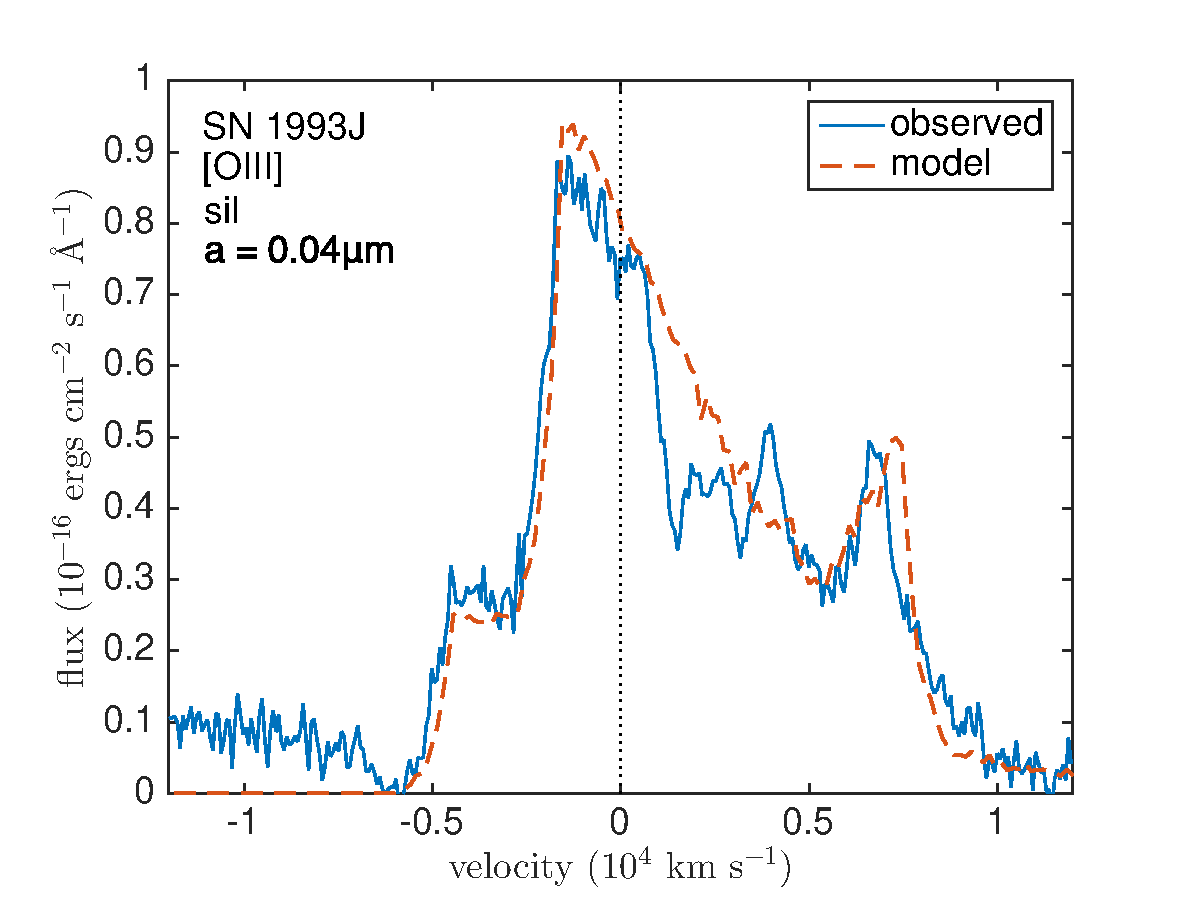
\includegraphics[scale=0.4,clip=true, trim=0 0 40 20]{chapters/chapter6/figs/93J/clumped/OIII_sil} \hspace{0.5mm}
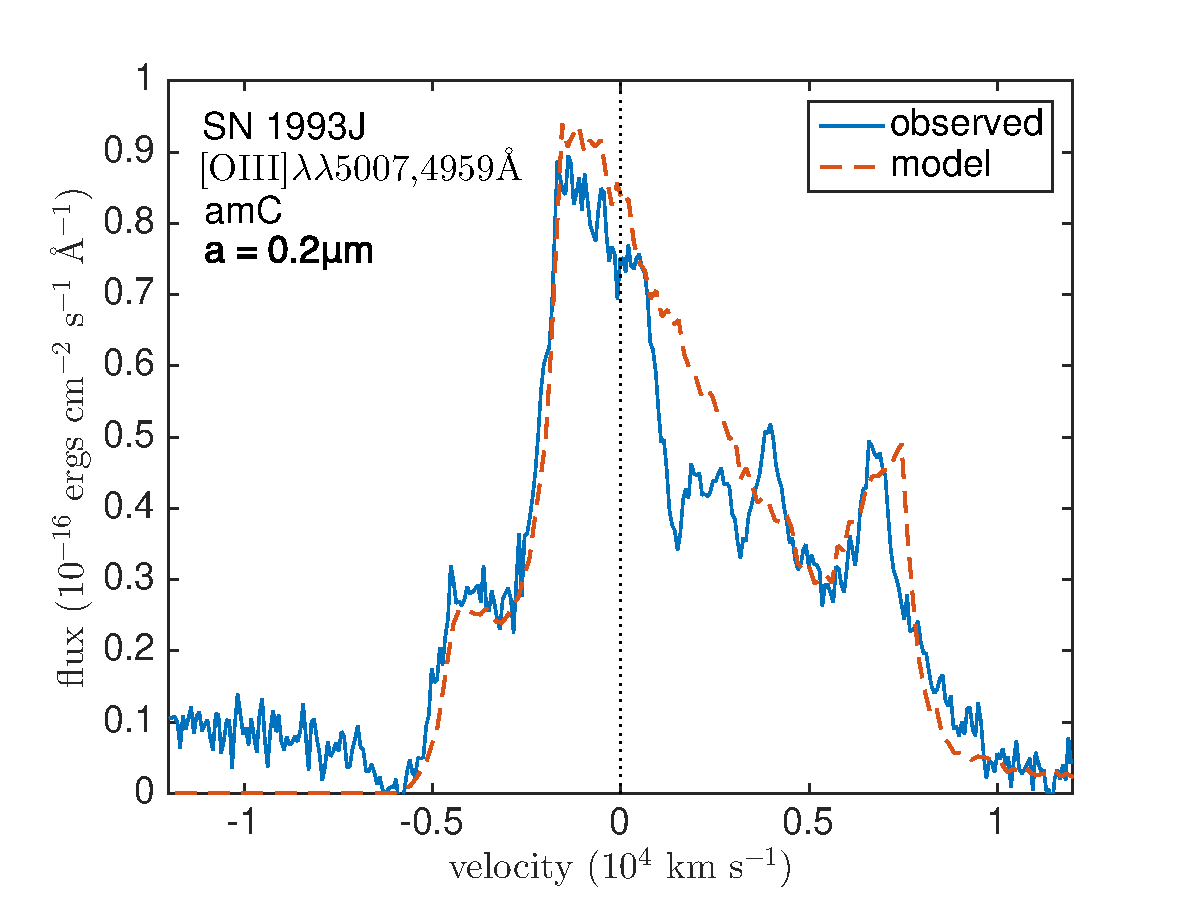
\includegraphics[scale=0.4,clip=true, trim=40 0 40 20]{chapters/chapter6/figs/93J/clumped/OIII_amC}

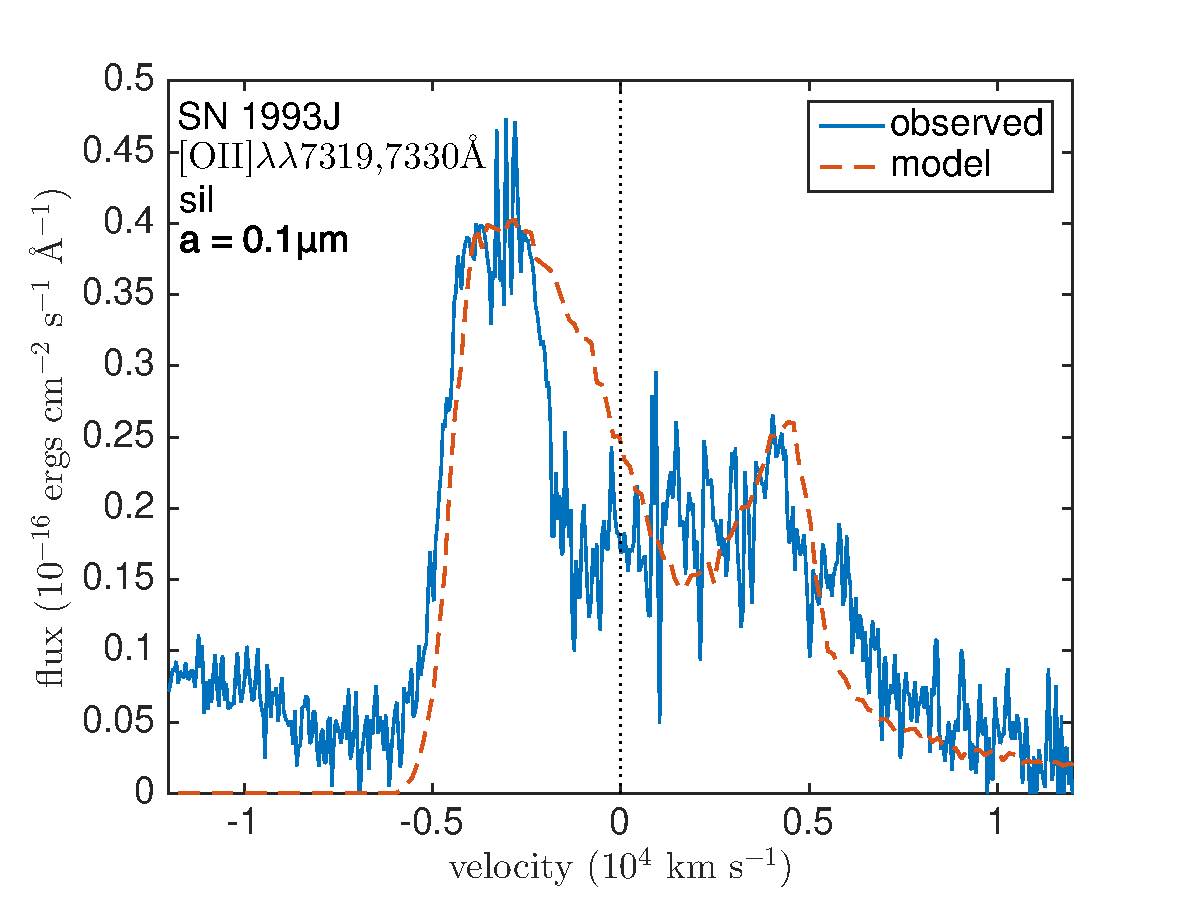
\includegraphics[scale=0.4,clip=true, trim=0 0 40 20]{chapters/chapter6/figs/93J/clumped/OII_sil}
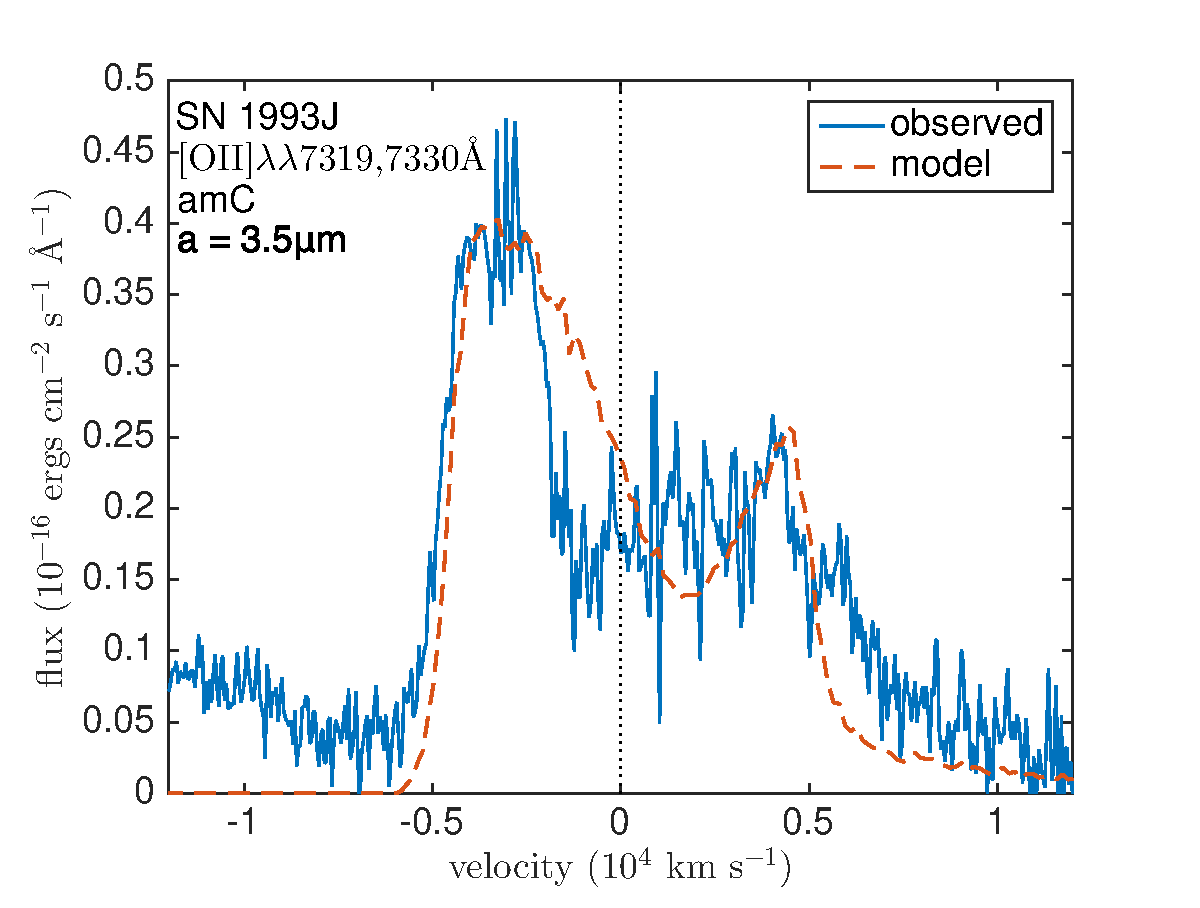
\includegraphics[scale=0.4,clip=true, trim=30 0 40 20]{chapters/chapter6/figs/93J/clumped/OII_amC}
\caption{Best clumped dust fits to the SN~1993J [O~{\sc iii}]$\lambda\lambda$5007,4959~\AA\ doublet ({\em top}) and the [O~{\sc ii}]$\lambda\lambda$7319,7330~\AA\ doublet  ({\em bottom}) for the parameters detailed in Table \ref{93J}.  For the [O~{\sc ii}] doublet, zero velocity was set at $\lambda=7319$~\AA\ and for the [O~{\sc iii}] doublet, zero velocity was set at $\lambda=4959$~\AA. Compositions and sizes are as detailed on the plots.}
\label{93J_clumped}
\end{figure}

A manual investigation of parameter space suggested that these issues with fitting the shape of the profile derived from the initial emissivity distribution.  The smooth nature of the emissivity distribution that I adopted could not reproduce the sharp downturn seen to the red side of the peak flux.  This could be due to an oxygen emission distribution that is potentially composed of a dense central region that produces the steep variations in the central regions with a more diffuse oxygen envelope accounting for the wings.  A different geometry may well alter the effects of scattering and could therefore reduce or remove the discrepancy in the required grain sizes.  I discuss these issues in further detail in Section \ref{scn:discuss93j}.

Parameters for the smooth dust models for [O~{\sc iii}]$\lambda\lambda$5007,4959~\AA\ and [O~{\sc ii}]$\lambda\lambda$7319,7330~\AA\   that are presented in Figure \ref{93J_smooth} are detailed in Table \ref{93J}. 
 
\subsection{SN~1993J Clumped Dust Models}

My clumped dust models of SN~1993J adopted the same clumped structure as for the SN~1980K clumped models and the SN~1987A clumped models ($f=0.1$ and $R_{clump}=R_{out}/25$).  All of the parameters were kept fixed from the smooth models except for the new clumped dust distribution.  Similar fits were found and the clumped geometry had little effect on the resultant modelled line profiles.   The required dust mass increased by a factor of approximately 1.5.  The clumped model parameters for the [O~{\sc iii}]$\lambda\lambda$5007,4959~\AA\ and [O~{\sc ii}]$\lambda\lambda$7319,7330~\AA\ fits that are presented in Figure \ref{93J_clumped} are detailed in Table \ref{93J}. 

\subsection{SN~1993J  Discussion}
\label{scn:discuss93j}
My models for the optical line profiles of SN~1993J do not fit the observed data quite as well as the models that I present in this thesis for other objects.  In particular, the modelled profiles tend to over-estimate the flux in the region just to the red side of the peak flux, where the observed profile exhibits a sharp downturn (see Figure \ref{boxy}).  The steepness of this drop cannot be matched by the models.  However, certain other features of the observed profiles are fitted well by the model.  For example, the [O~{\sc iii}]$\lambda\lambda$5007,4959~\AA\  model line profile in particular fits bumpy features on both the red and blue sides of the profile at approximately $-4000$~km~s$^{-1}$ and $+6000$~km~s$^{-1}$ quite well.  The bump near $+6000$~km~s$^{-1}$ is simply a due to absorption in the region between $-V_{min}$ and $+V_{min}$ causing a peak at the location of the minimum velocity (for the 5007~\AA\ component).  The small discrepancy in the location of the [O~{\sc iii}] peak at around $\sim+6000$~km~s$^{-1}$ may be a result of a net velocity shift of the supernova away from the observer (see Section \ref{scn:CasA_smooth} for a discussion of this effect in more detail) or a discrepancy between the smooth, symmetrical models and a more clumpy, asymmetrical geometrical structure for the remnant \citep{Tran1997}.  Similarly, the difference in the grain sizes, and hence the dust masses, required to fit the [O~{\sc iii}] and [O~{\sc ii}] lines (see Table \ref{93J}) might also indicate the need for a different distribution of dust or gas.  The bumpy features seen in these lines were discussed by \citet{Matheson2000b} who postulated the possibility that the `double-horned' shape was a consequence of the ejecta colliding with a disk-like or flattened region. While it is possible that the blue-shifted asymmetry observed in the optical line profiles is not a result of dust in the ejecta, given how well certain aspects of the observed profiles are fitted, it seems more likely that it is simply the case that a more complex geometry is required for the dust models to better fit the data.

\citet{Houck1996} discussed the spectra of SN~1993J at somewhat earlier times than I consider here (140--416 days).  The asymmetries that are present in the oxygen lines that I model here were also present at earlier times.  \citet{Houck1996} suggested that  this asymmetry could be explained by interaction between the lines.  In particular, they discussed the effects of scattering by H$\alpha$ on the [O~{\sc i}]$\lambda\lambda$6300,6363~\AA\ line profile.  It is possible that line blending affects the resultant profile, and it is logical that scattering by H$\alpha$ might cause the sharp drop in the line profile of [O~{\sc i}] that is seen on the red side.  However, the similarities between the very late-time line profiles of [O~{\sc i}]$\lambda\lambda$6300,6363~\AA\ and [O~{\sc ii}]$\lambda\lambda$7319,7330~\AA\ would suggest that  the cause of this drop is more likely related to the geometrical structure of the emitting region rather than interaction with nearby lines.  Additionally, the line optical depths are much smaller at late epochs and therefore H$\alpha$ scattering is very unlikely to account for this feature at late epochs.

\citet{Nomoto1993} produced a number of explosion models of a helium star as an analogue for a Type IIb supernova such as SN~1993J.  From one of their models (4H47), they presented the  distribution of different elements throughout the expanding shell.  As might be predicted from the line profiles, the oxygen is located in two distinct regions with significantly different densities (see Figure \ref{4h47}).   The distribution of the oxygen in the models is smooth and it seems likely that my overestimation of the flux just to the red side of the peak could well be resolved by considering a two-component density distribution such as this.

\begin{figure}
\centering
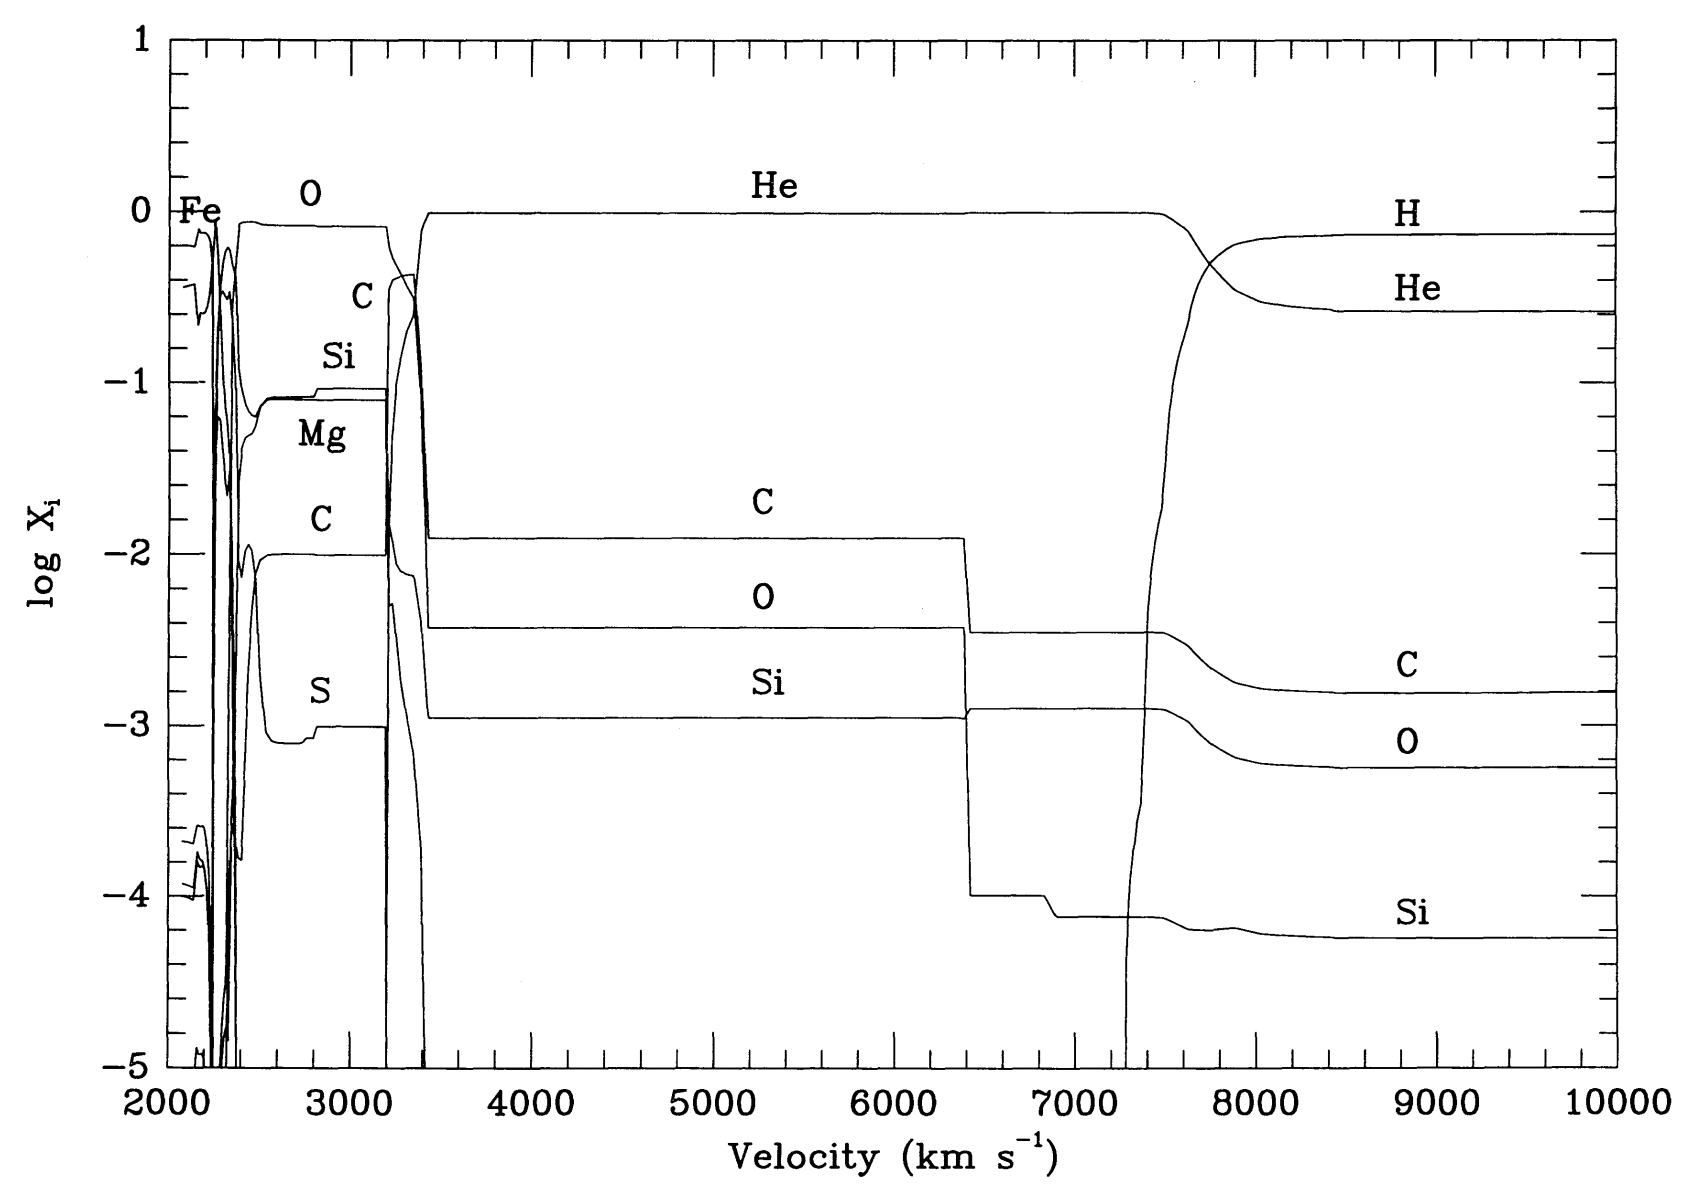
\includegraphics[scale=0.4,clip=true, trim=30 0 0 0]{chapters/chapter6/figs/93J/explosion_model.png}
\caption{Composition of model 4H47 as a function of expansion velocity as computed by \citet{Nomoto1993}.  Image taken from \citet{Houck1996}.}
\label{4h47}
\end{figure}

It should also be noted that SN~1993J had a particularly unusual red supergiant progenitor with a postulated stripped envelope caused by the presence of a B-star binary companion \citep{Maund2004,Fox2014} and resulting in a significant mass of circumstellar material surrounding the supernova.  Photometric analyses performed by \citet{Zhang2004} suggest that the late-time optical emission from SN~1993J is largely powered by interaction between the blast wave and the circumstellar material.  In this case, the geometry of the emitting regions is especially complex, and may in particular account for the significant substructure seen in the optical line profiles.

For both SN~1980K and SN~1993J, the effects of including a clumped dust distribution in the models rather than a smooth dust distribution  increased the required dust mass by a factor of approximately 1.5, very similar to the factor found for SN~1987A from the models presented in the previous chapter.  In these cases, the clumped geometry has little effect on the resulting profiles except to reduce the degree of absorption.  The extent of the extended red scattering wing is also somewhat reduced by dust clumping.


\section{Cassiopeia A}
\label{CasA_intro}

Cassiopeia~A (Cas~A) is a Milky Way supernova and is a fairly unusual object.  It is extremely close at only 3.4~kpc away \citep{Reed1995} and is rather large measuring around 4~pc in diameter \citep{Hurford1996}.  There have not been any records found of its detection around the time of its explosion.  However, analysis of its expansion velocities and geometry have allowed its explosion date to be determined to be approximately 1681$\pm$19CE \citep{Fesen2006} making the supernova remnant approximately 330 years old.  Cas~A is the strongest radio source in the sky outside of the solar system and was initially discovered at radio wavelengths in the 1940s.  Since then, it has been well observed across the entire wavelength range.  Recent spectroscopic observations in the near-IR of light echoes caused by the reflection of early light from the supernova off surrounding interstellar dust have allowed the original supernova explosion to be classified.  This work has suggested that Cas~A was the result of a Type IIb supernova explosion with a likely progenitor stellar mass of $\sim15-20$~M$_{\odot}$ \citep{Krause2008}.

In Chapter \ref{chp:chp1}, I discussed the importance of Cas~A to our understanding of dust formation in supernovae and their remnants.  \citet{Barlow2010} present a brief review of the ejecta dust mass estimates in Cas~A up to 2010.  Early dust mass estimates were largely based on observations of the warm dust component in the ejecta.  \citet{Arendt1999} estimated a mass of 0.038~M$_{\odot}$ of 52 K dust based on fitting IRAS 60~$\mu$m and 100~$\mu$m fluxes.  A similar mass of $0.020-0.054$~M$_{\odot}$ of warm dust at $65-265$K was estimated to be emitting between 5~$\mu$m and 70~$\mu$m by \citet{Rho2008}, particularly in a bright ring associated with the reverse shock.   \citet{Arendt2014} used {\em Spitzer} observations to derive a  mass of $\sim$0.04~M$_{\odot}$ of warm dust.  Observations at longer wavelengths of the cold dust in the ejecta have led to higher dust mass estimates with \citet{Dunne2003} using SCUBA data to estimate a dust mass of between $2-4$~M$_{\odot}$.  This was contested by \citet{Krause2004} who suggested that the majority of this emission could be from cold dusty clouds located along the line of sight to Cas~A and placed an upper limit of 0.2~M$_{\odot}$ of cold dust in the ejecta.  However, observations of strongly polarised emission at long wavelengths obtained using the SCUBA polarimeter have been used to argue for the presence of an ejecta-condensed cold dust mass of $\sim1$~M$_{\odot}$ \citep{Dunne2009}.  Modelling by \citet{Nozawa2010}  reproduced the observed IR SED using 0.08~M$_{\odot}$ of dust, of which 0.072~M$_{\odot}$ was inside the reverse shock.  They could not isolate a cold dust component to be within the ejecta but estimated its mass to be $\sim0.06$~M$_{\odot}$.  Sub-mm observations by \citet{Sibthorpe2010} using SCUBA and by \citet{Barlow2010} using {\em Herschel} led to estimates for a cool ($T\sim35$K)  dust component associated with the remnant of 0.06~M$_{\odot}$ and 0.075$\pm$0.028~M$_{\odot}$ of silicate dust respectively. 

More recently, {\em Spitzer} and {\em Herschel} studies of the mass and composition of dust in Cas~A has suggested that the total  mass of dust with $T\geqslant35$K present in the ejecta is of the order of $\sim0.1$~M$_{\odot}$ \citep{Barlow2010,Nozawa2010,Arendt2014} with strong foreground emission from cold interstellar dust making it difficult for {\em Herschel} to detect colder dust within the remnant.  Given the difficulties in modelling this object, it is perhaps not surprising that there is significant variation in the estimates of the dust mass in the ejecta with previous estimates covering a wide range, from less than $3\times10^{-3}$~M$_{\odot}$ \citep{Dwek2004} to greater than $4$~M$_{\odot}$ (\citealt{Dunne2003,Dunne2009}; but see also \citealt{Krause2004}).  



\begin{figure}
\centering
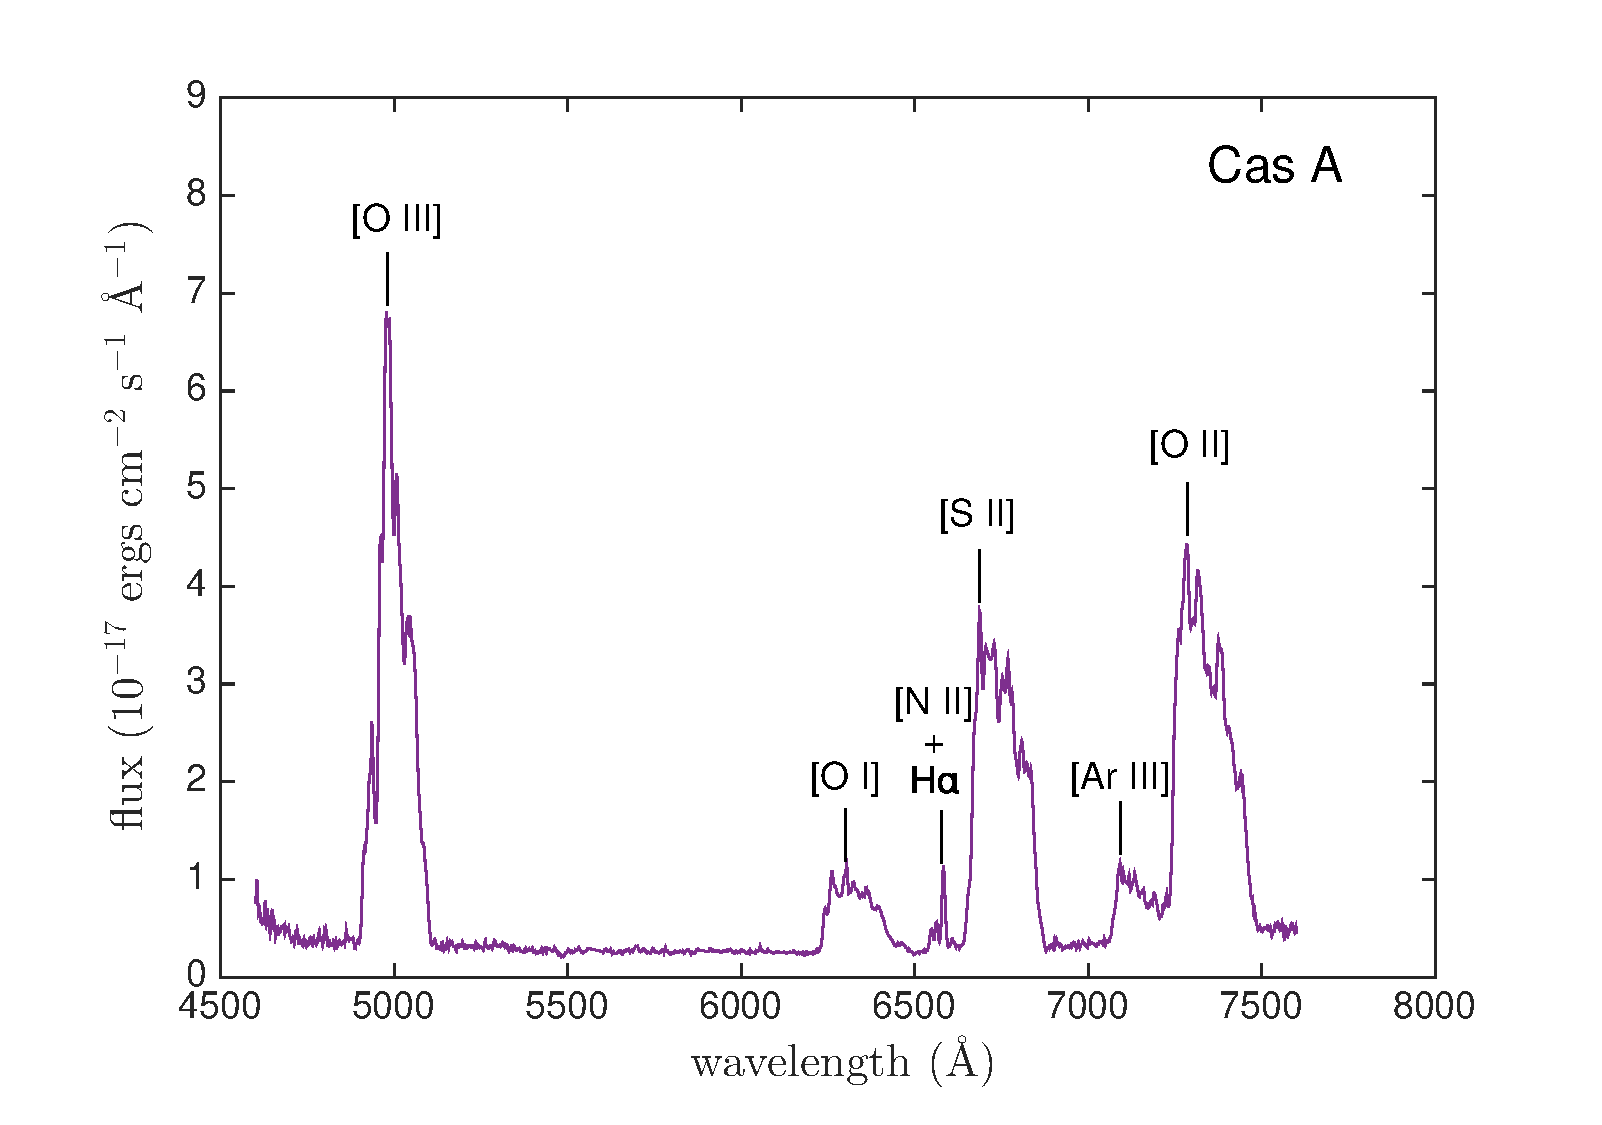
\includegraphics[clip=true,scale=0.6, trim=30 0 50 20]{chapters/chapter6/figs/CasA/spectrum}
\caption{The integrated spectrum of Cas A \citep{Milisavljevic2013}.}
\label{CasA_spectrum}
\end{figure}

The integrated optical spectrum of Cas~A \citep{Milisavljevic2013} reveals red-blue asymmetries in many of the  line profiles.  In particular, the oxygen lines [O~{\sc i}]$\lambda\lambda$6300,6363~\AA, [O~{\sc ii}]$\lambda\lambda$7319,7330~\AA\  and [O~{\sc iii}]$\lambda\lambda$5007,4959~\AA\ exhibit a blue-shifted asymmetry, with the [O~{\sc iii}] doublet especially demonstrating a strong blueshift with considerable substructure.  I have modelled all three of these features with a primary focus on the [O~{\sc iii}] doublet.

\subsection{The Integrated Optical Spectrum of Cas~A}

The integrated spectrum of Cas~A presented in Figure \ref{CasA_spectrum}, from \citet{Milisavljevic2013}, was kindly provided to me by Dr Dan Milisavljevic.  It is composed of observations from a series of observing runs between September 2007 and November 2010 that were conducted in order to obtain low-dispersion optical spectra across the remnant.  The majority of observations were carried out at the MDM Observatory at Kitt Peak, Arizona using the 2.4m Hiltner telescope and the Mayall 4m telescope.  The MDM Modular Spectrograph was used with an `Echelle' detector.  A long slit of dimensions $2''\times5'$ was used and was oriented North-South.  Exposure times were generally 2$\times$500s.  The wavelength range covered was 4500--7000~\AA\  with a spectral resolution of 6~\AA.  
%A few of the observations of the main shell of Cas~A used alternative spectrographs (the Mark III Spectrograph and the Chivens CCD Spectrograph).  The lowest spectral resolution of any spectrum observed was 12~\AA.  
The integrated spectrum was ultimately composed of 80 long slit spectra spaced 3" apart across the entire main shell which is approximately $4'$ in diameter.  The slit positions are shown in Figure \ref{CasA_slit_positions}.  Assuming an explosion date of 1681, Cas~A was nearly 330 years old at the time that the spectra were acquired.


\subsection{Smooth Dust Models for the Oxygen Lines of Cas A}
\label{scn:CasA_smooth}
The modelling of the Cas~A spectrum was initially focussed on the [O~{\sc iii}]$\lambda\lambda$5007,4959~\AA\  doublet, which exhibits a pronounced asymmetry.  The process of finding a fit to the line profile was the same as described in Sections \ref{results} and \ref{CasA_OIII}, i.e. the maximum velocity was identified from the point at which flux vanishes on the blue side, the inner to outer radius ratio determined from various inflection points and the density profile determined from the shape of the profile.  The other parameters were then iterated over to find the best fitting profile.  

\begin{figure}
\centering
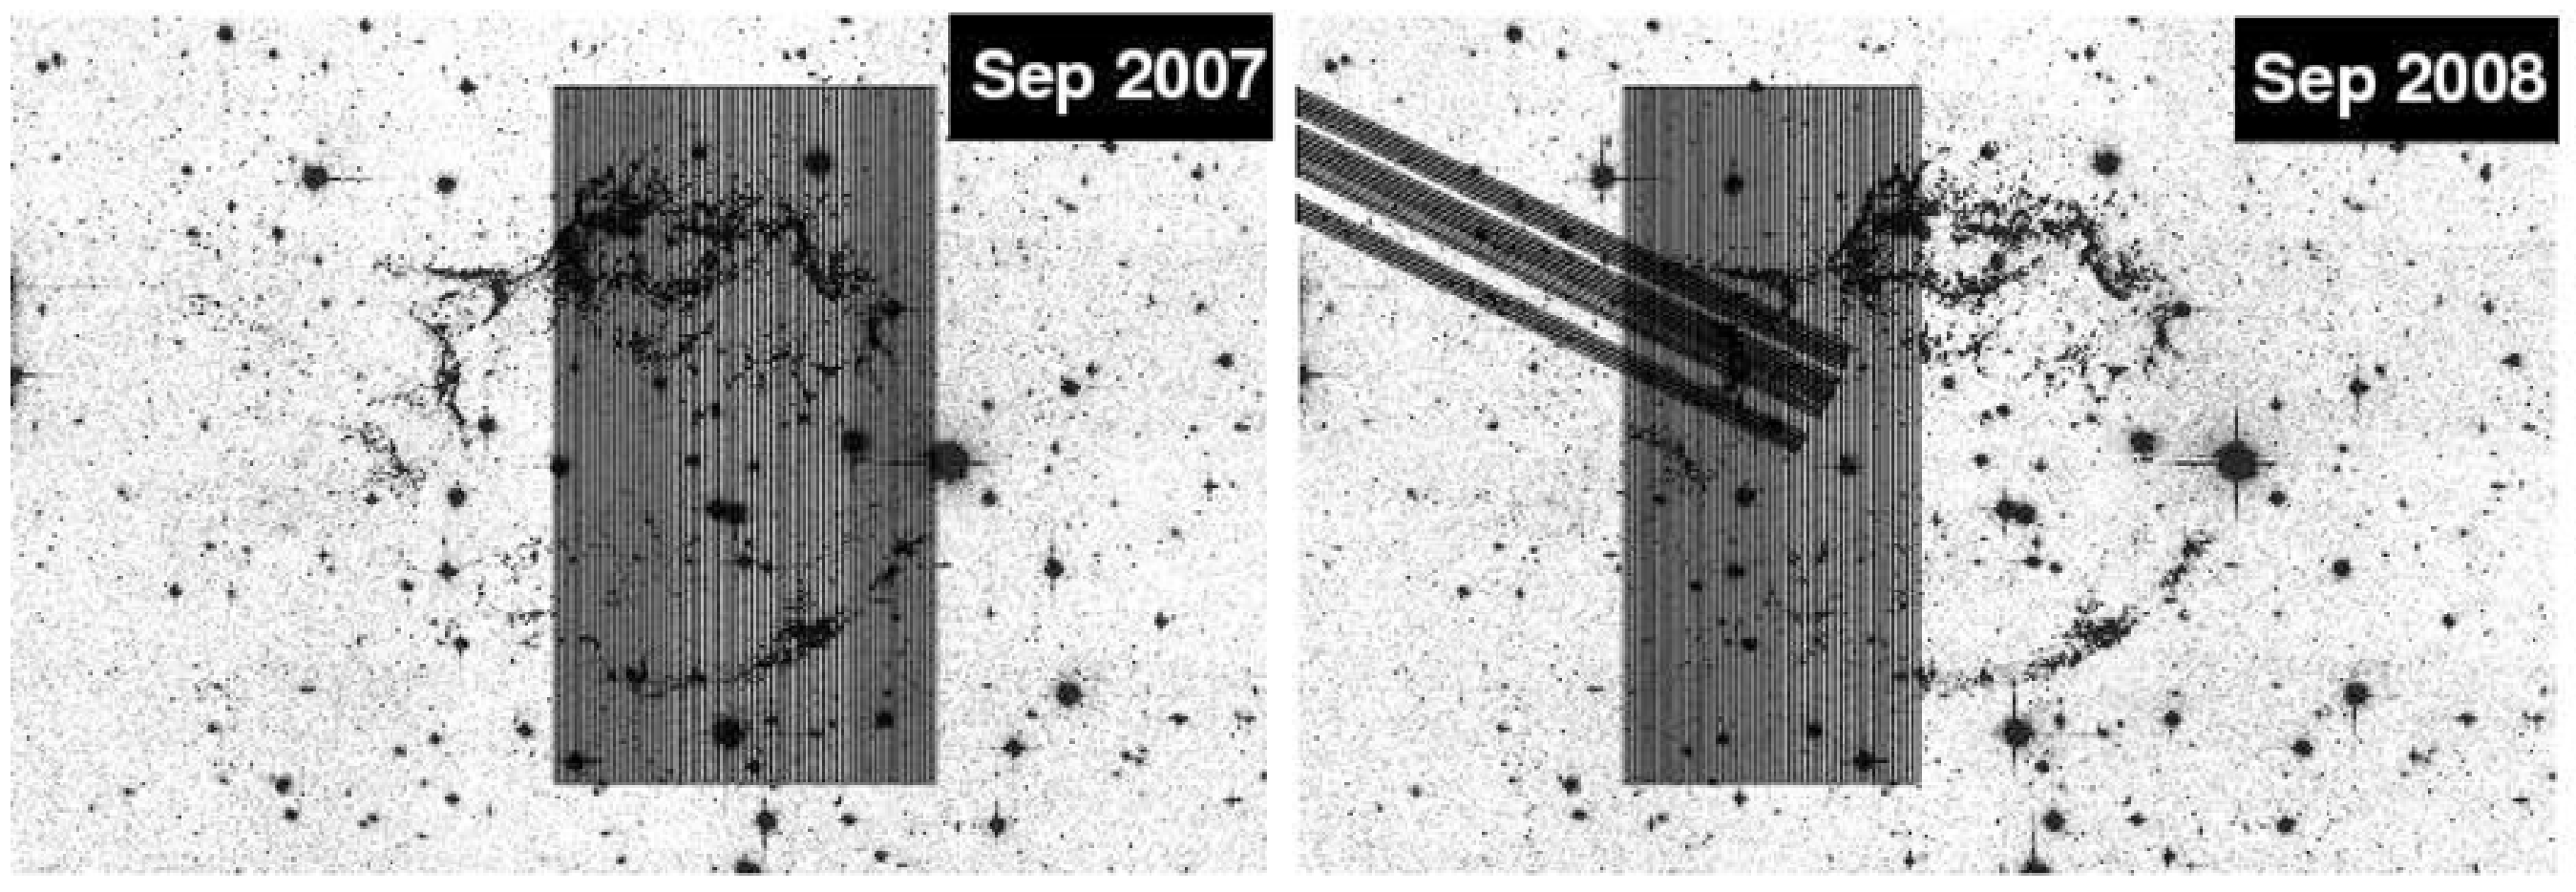
\includegraphics[clip=true,scale=0.3, trim=0 0 0 0]{chapters/chapter6/figs/CasA/slit_positions.png}
\caption{Finding charts of the long-slit positions used to compose the integrated spectrum of the main shell of Cas~A.  The background image is a mosaic created from 2004 HST/ACS observations \citep{Fesen2006a}.  Image is taken from \citet{Milisavljevic2013}.}
\label{CasA_slit_positions}
\end{figure}

I managed to produce a reasonable fit to the data using the parameters listed in the first row of Table \ref{CasA_smooth_params}.  The profile is presented in the left pane of Figure \ref{CasA_OIII}.  As can be seen,  the modelled line profile generally fits the observed line profile quite well, although it fails to fit the red side of the profile adequately.  A thorough, manual investigation of parameter space resulted in the conclusion that the profile was much better fitted if the entire modelled profile was shifted to the red by $+700$~km~s$^{-1}$.  This might well be a reasonable assumption.  Cas~A is known to be significantly asymmetrical \citep{Rest2011} with radial velocities spanning -4000 to +6000~km~s$^{-1}$ \citep{Milisavljevic2013} suggesting that the net line-of-sight velocity is likely away from the observer and indicating the need for an overall velocity shift to correct for this.  I found that models of the  [O~{\sc ii}]$\lambda\lambda$7319,7330~\AA\ and [O~{\sc i}]$\lambda\lambda$6300,6363~\AA\  lines were also substantially improved if the entire model profile was allowed to be uniformly shifted towards the red.  For the remainder of the models I therefore shifted the profiles in velocity space to better fit the data based on the likelihood that the sampled emitting regions had an overall net velocity away from the observer.  Fits to the line profiles were significantly improved following this translation (see Figures \ref{CasA_OIII} to \ref{CasA_OIII_clumped}).



A model of the shifted [O~{\sc iii}]$\lambda\lambda$5007,4959~\AA\  line is presented in Figure \ref{CasA_OIII} and the parameters used for this model are presented in the second row of Table \ref{CasA_smooth_params}.  A total dust optical depth of $\tau=0.49$ at 5007~\AA\  between $R_{in}$ and $R_{out}$ was found to best fit the profile.  An albedo of $\omega\approx0.15$ at 5007~\AA\  was also necessary to increase the flux on the far red side of the profile.

\afterpage{
\begin{landscape}
\centering
\setlength{\tabcolsep}{10pt}
\begin{table}
\centering
%	\begin{minipage}{180mm}
	\caption{The parameters used for the smooth models of Cas~A with a medium composed of 50\% amorphous carbon and 50\% silicate grains of radius $a=0.05~\mu$m.  Optical depths are given from $R_{in}$ to $R_{out}$ at $\lambda = 5007$~\AA\  for [O~{\sc iii}], $\lambda = 7319$~\AA\  for [O~{\sc ii}] and $\lambda = 6300$~\AA\  for [O~{\sc i}].  The doublet ratio is always the ratio of the stronger line to the weaker line. The asterisk indicates that the parameters listed describe the gas density distribution.  The dust density distribution is the same in all cases (as detailed for the shifted [O~{\sc ii}] doublet in the second row).}
	\label{CasA_smooth_params}
	\centering
  	\begin{tabular}{@{} cccccccccccc @{}}
    	\hline
  &$v$ shift& $V_{max}$ & $V_{min}$ & $R_{in}/R_{out}$ & $\beta$ & $M_{dust}$ & $R_{out}$ & $R_{in}$ & doublet  & $\tau_{\lambda}$   \\
	& (km~s$^{-1}) $& (km~s$^{-1} $)& (km~s$^{-1} $) & & & ($M_{\odot}$) & (10$^{18}$cm) & (10$^{18}$cm) & ratio \\
	\hline
[O~{\sc iii}]  & 0 & 4500 & 1800 & 0.4  & 2.0 & 0.9 & 4.7 & 1.9 & 2.98 & 0.53  \\ \relax
[O~{\sc iii}]  & +700 & 5000 & 2500 & 0.5  & 2.0 & 1.1 & 5.2 & 2.6 & 2.98 & 0.49  \\ \relax
[O~{\sc ii}]*  & +1000 & 5000 & 3250 & 0.65  & 2.0 & 1.1 & 5.2 & 3.4 & 1.23 & 0.21  \\ \relax
[O~{\sc i}]*  & +1000 & 5000 & 3250 & 0.65  & 2.0 & 1.1 & 5.2 & 3.4 & 3.1 & 0.30  \\ 
    \hline
  \end{tabular}

%\end{minipage}
\end{table}
\end{landscape}
\begin{figure}
\centering
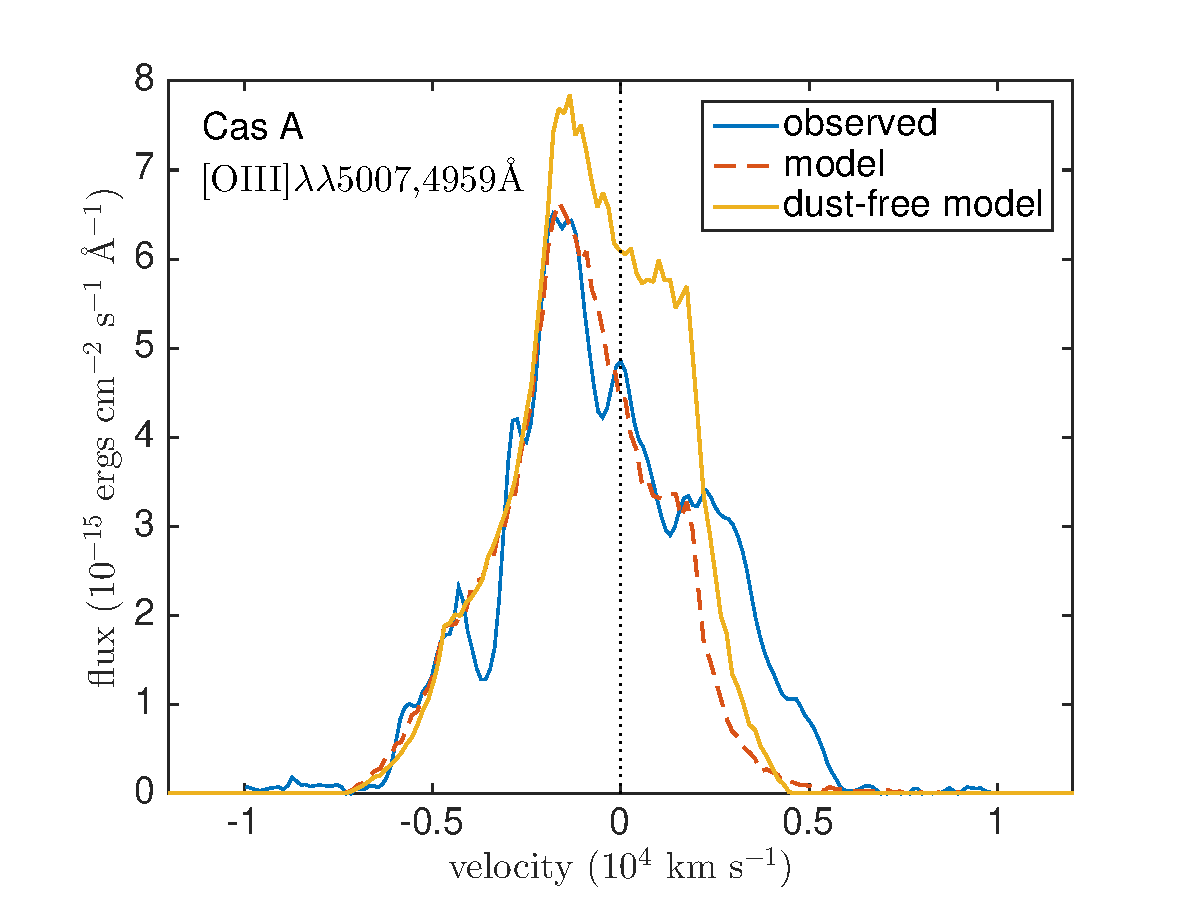
\includegraphics[scale=0.43,clip=true, trim=30 0 50 20]{chapters/chapter6/figs/CasA/CasA_OIII}
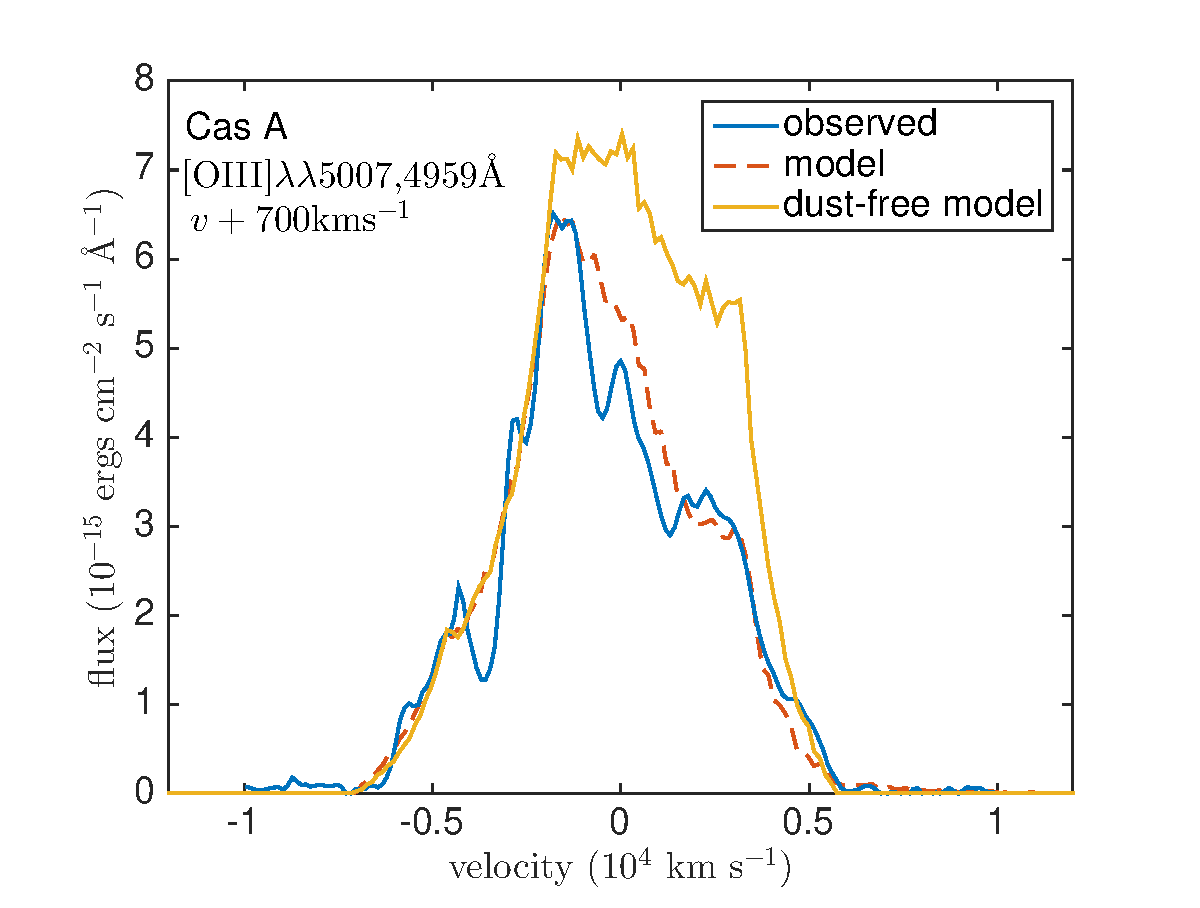
\includegraphics[scale=0.43,clip=true, trim=30 0 50 20]{chapters/chapter6/figs/CasA/CasA_shifted_OIII}
\caption{Best smooth dust fits to the Cas~A [O~{\sc iii}]$\lambda\lambda$5007,4959~\AA\ doublet for the parameters detailed in Table \ref{CasA_smooth_params}.  On the left is the original [O~{\sc iii}] line profile and on the right the model [O~{\sc iii}] line has been shifted uniformly towards the red by $+700$~km~s$^{-1}$. Zero velocity was set at $\lambda=5007$~\AA.}
\label{CasA_OIII}
\end{figure}
}

The composition of the dust has a significant effect on the overall dust mass for this optical depth and albedo.  An attenuated line profile model of the [O~{\sc iii}]$\lambda\lambda$5007,4959~\AA\  doublet  from Cas~A could not be found using 100\% astronomical silicate dust \citep{Draine1984}.  There is little to no red scattering wing seen, hence the relatively low value of $\omega$, and therefore relatively small silicate grains would be required to reproduce the red side of the profile.  Silicate grains of this size have extremely low optical absorption efficiencies and therefore the best-fitting optical depth of $\tau=0.49$ would correspond to an implausibly large mass of dust ($>20$~M$_{\odot}$) if it was composed entirely of astronomical silicates.



The chemical composition of the dust in the ejecta of Cas~A is known to be extremely complex \citep{Rho2008,Arendt2014} with many different species of dust grain present in the ejecta.  The presence of silicate dust has been deduced based on typical silicate emission features observed in the mid-IR region of the spectrum \citep{Rho2008}.  However, the likelihood of the presence of a variety of other species has been discussed \citep{Arendt2014}. In Table \ref{CasA_dust_masses}, I detail the dust masses required to fit the [O~{\sc iii}]$\lambda\lambda$5007,4959~\AA\  line profile for different fractions of silicates and amorphous carbon grains for a single grain size.  For each composition I determined the grain radius based on the albedo necessary to fit the profile ($\omega\approx0.15$) and then varied the dust mass to achieve the required optical depth.  The derived dust masses cover a wide range of values, between $0.37 - 6.5$~M$_{\odot}$.   

It might have been possible  to determine the approximate composition based on the relative optical depths necessary to fit different blue-shifted lines in the spectrum and the wavelength dependence of dust absorption for different compositions.  I therefore considered fitting the blue-shifted [O~{\sc ii}]$\lambda\lambda$7319,7330~\AA\  and [O~{\sc i}]$\lambda\lambda$6300,6363~\AA\  lines from Cas~A.  Unfortunately, at the small grain sizes required, there is not significant variation in the relationship between the absorption efficiencies at 5007~\AA\  and 7319~\AA\  for different dust compositions and I could not  therefore determine the composition via this approach in this case.  Additionally, the [O~{\sc ii}] and [O~{\sc i}] lines are much less sensitive to variations in both density distributions and dust mass, partly due to the high frequency of bumpy features observed in these lines which contaminate the intrinsic broad profile.  The best-fitting models for these lines were therefore quite degenerate i.e. there were multiple sets of parameters that resulted in reasonable fits.  
\begin{figure}
\centering
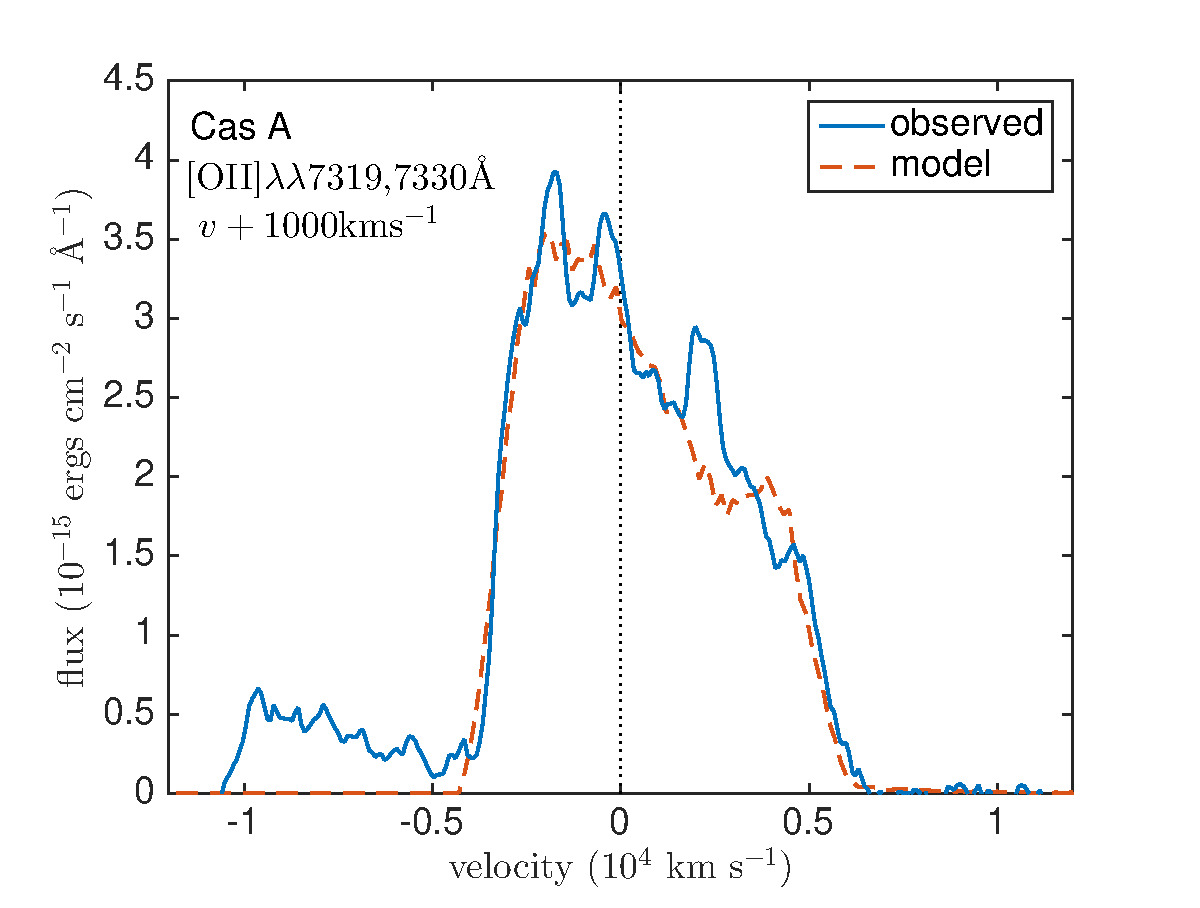
\includegraphics[scale=0.41,clip=true, trim=15 0 40 20]{chapters/chapter6/figs/CasA/CasA_shifted1000_OII}
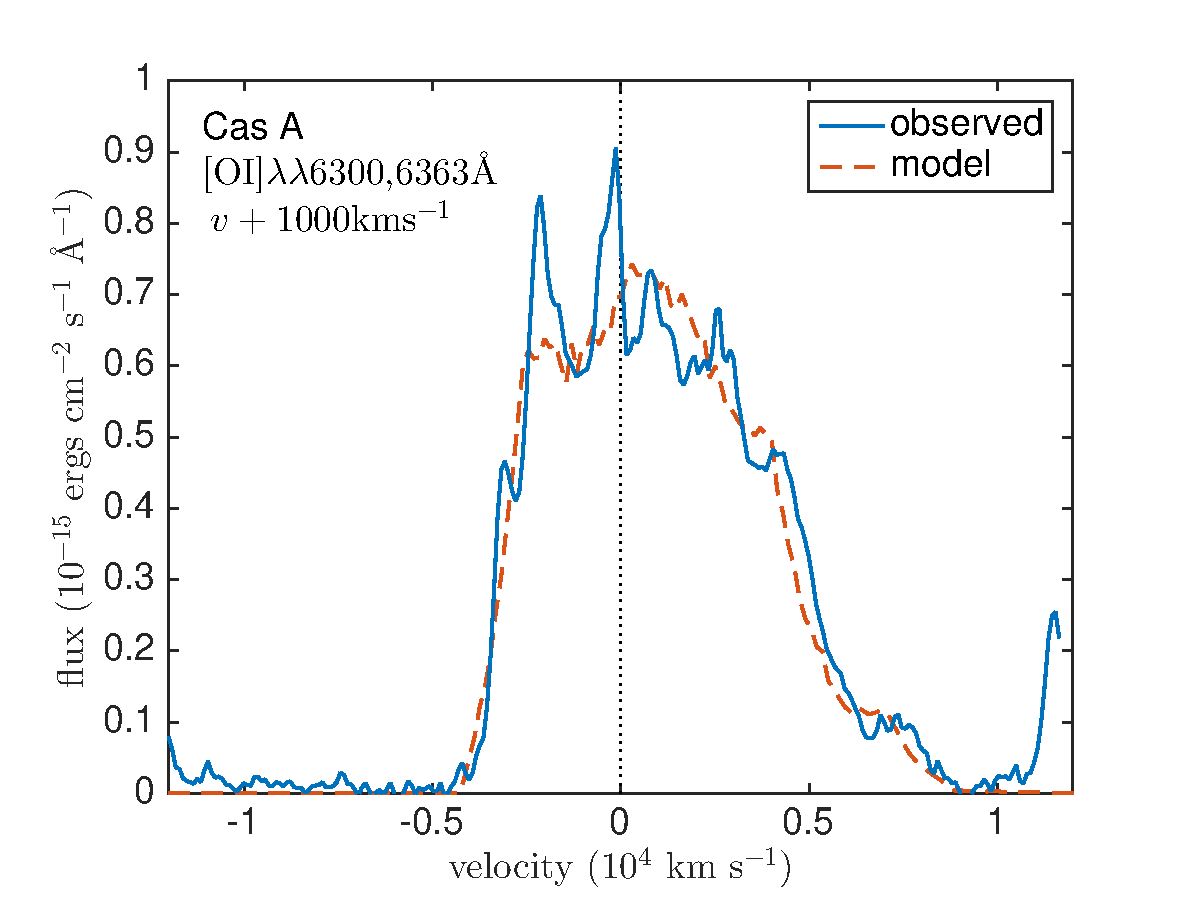
\includegraphics[scale=0.41,clip=true, trim=15 0 40 20]{chapters/chapter6/figs/CasA/CasA_OI_shifted1000}
\caption{Best smooth dust fits to the Cas~A [O~{\sc ii}]$\lambda\lambda$7319,7330~\AA\  doublet ({\em left}) and the [O~{\sc i}]$\lambda\lambda$6360,6363~\AA\  doublet ({\em right}) for the parameters detailed in Table \ref{CasA_smooth_params} along with the intrinsic dust-free profile.  Both model line profiles have been shifted uniformly towards the red by $+1000$~km~s$^{-1}$.}
\label{CasA_OI_OII}
\end{figure}

However, it was possible to use these lines to determine the reliability of the best-fitting model for the  [O~{\sc iii}]$\lambda\lambda$5007,4959~\AA\  line profile.  I adopted the dust distribution determined using the [O~{\sc iii}] fits and investigated models for the [O~{\sc ii}]$\lambda\lambda$7319,7300~\AA\  and [O~{\sc i}]$\lambda\lambda$6300,6363~\AA\  profiles to see if this dust distribution was capable of fitting these lines as well.  I adopted an emissivity distribution that was slightly different to the [O~{\sc iii}] line (see Table \ref{CasA_smooth_params}) and shifted the observed line profiles by $-1000$~km~s$^{-1}$.  These emissivity distributions were then modelled with the dust distribution and dust mass for the best-fitting smooth [O~{\sc iii}] model.  The resultant [O~{\sc ii}] and [O~{\sc i}] line profiles are very good fits (see Figure \ref{CasA_OI_OII}).  This suggests that the models are consistent and, if the relative abundance of dust grain species present in the ejecta can be determined via other means, that the dust mass can be well-constrained using this method.  All of the line profile models listed above adopted intrinsic doublet strengths from \citet{Zeippen1987} and \citet{Storey2000}.  



\subsection{Clumped Dust Models for  the Oxygen Lines of Cas A}

The ejecta of Cas~A is highly clumped \citep{Fesen2001}.  Recently, models by \citet{Biscaro2014} have suggested that dust cannot in fact form in the gas phase in the ejecta of Cas~A unless extremely dense knots of material are present.  It is therefore important, as with SN~1987A, to consider the effects of clumping on the line profiles.  I continue to focus on the [O~{\sc iii}] line profile from Cas~A in considering the effects of clumping.  Clearly, the ejecta has a complex geometry with many clumps of different sizes and likely different ionisation states and dust species within each.  The models that I present here are included to give some indication of the effects of clumping within the ejecta rather than to be representative of the state of the ejecta at this time.  To this end I present a number of models of the [O~{\sc iii}] line profile based on the smooth dust fits that I presented in the previous section.  I consider two different clump sizes, ones with width $R_{out}/25$ and ones with width $R_{out}/10$.  I also consider three different clump volume filling factors $f=0.05$, $f=0.1$ and $f=0.25$.  For each combination of clump size and filling factor I evaluate the required increase or decrease in the dust mass over the smooth dust model.  All other parameters were kept fixed such that packets were emitted  according to the smooth distribution and geometry described by the parameters listed in Table \ref{CasA_smooth_params}.
\begin{table}
\centering
%	\begin{minipage}{180mm}
	\caption{The variation in dust mass for a fixed optical depth $\tau_{5007~\AA}=0.49$ for the parameters listed in Table \ref{CasA_smooth_params}.}
	\label{CasA_dust_masses}
	\centering
  	\begin{tabulary}{12cm}{C C C C}
    	\hline
	\% silicate  & \% amorphous & grain radius $a$ &  $M_{dust}$ \\
	grains& carbon grains&($\mu$m)&(M$_{\odot}$)\\
		\hline
90	&10	&0.035&	6.5 \\
75	&25	&0.04	&2.5\\
50	&50	&0.045&	1.1\\
25	&75	&0.048&	0.6\\
0	&100	&0.05&	0.37\\
    \hline
  \end{tabulary}
\end{table}

\begin{figure}
\centering
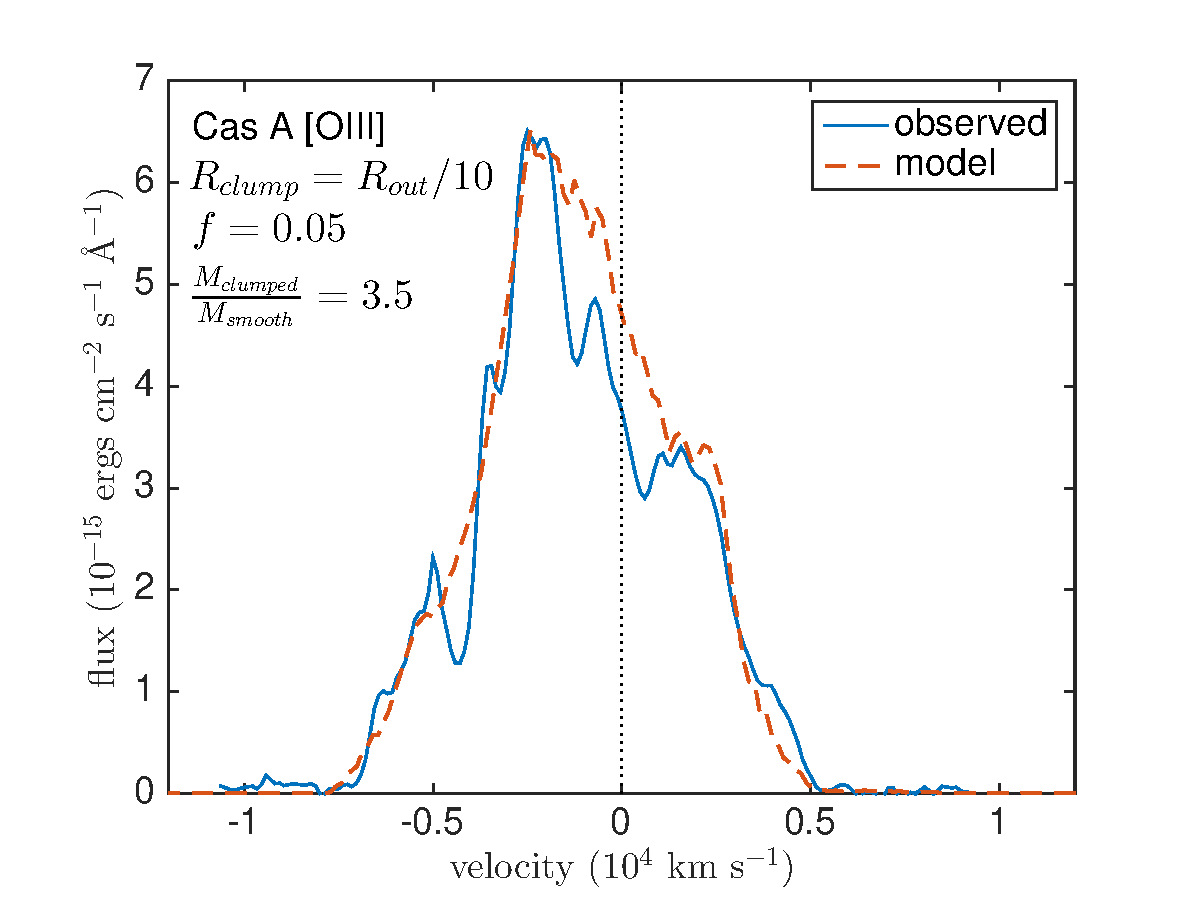
\includegraphics[scale=0.43,clip=true, trim=30 0 50 20]{chapters/chapter6/figs/CasA/clumped/CasA_OIII_c10_f0_05}
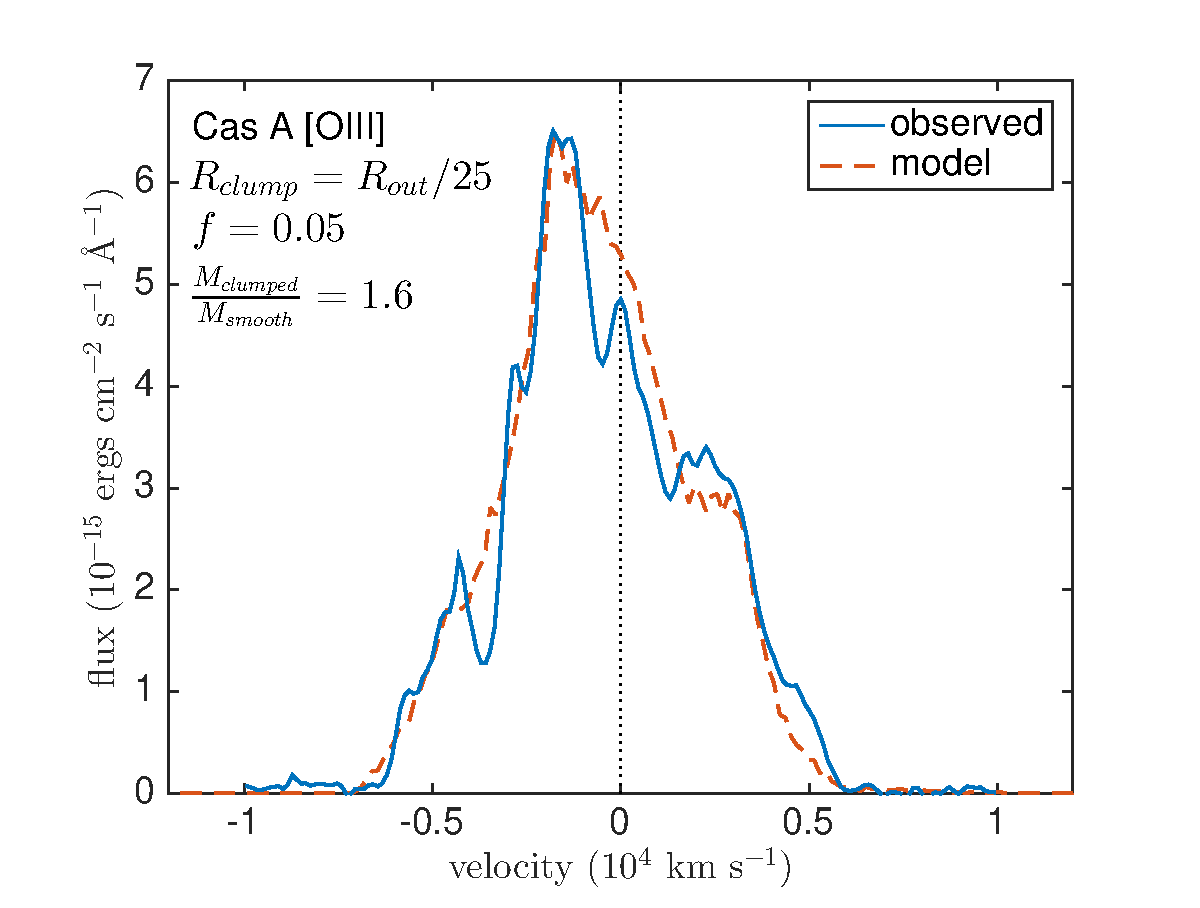
\includegraphics[scale=0.43,clip=true, trim=30 0 40 20]{chapters/chapter6/figs/CasA/clumped/CasA_OIII_c25_f0_05}

\vspace{6mm}
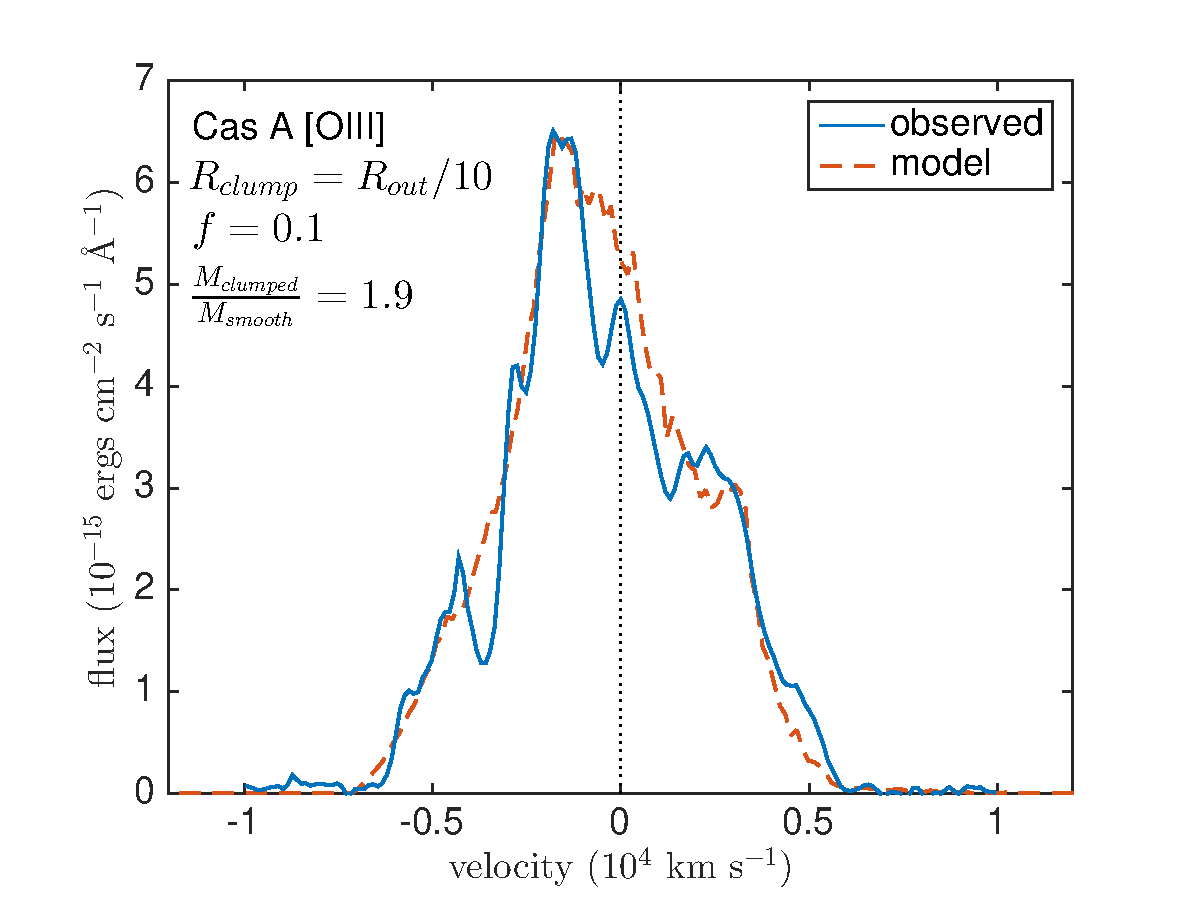
\includegraphics[scale=0.43,clip=true, trim=30 0 50 20]{chapters/chapter6/figs/CasA/clumped/CasA_OIII_c10_f0_1}
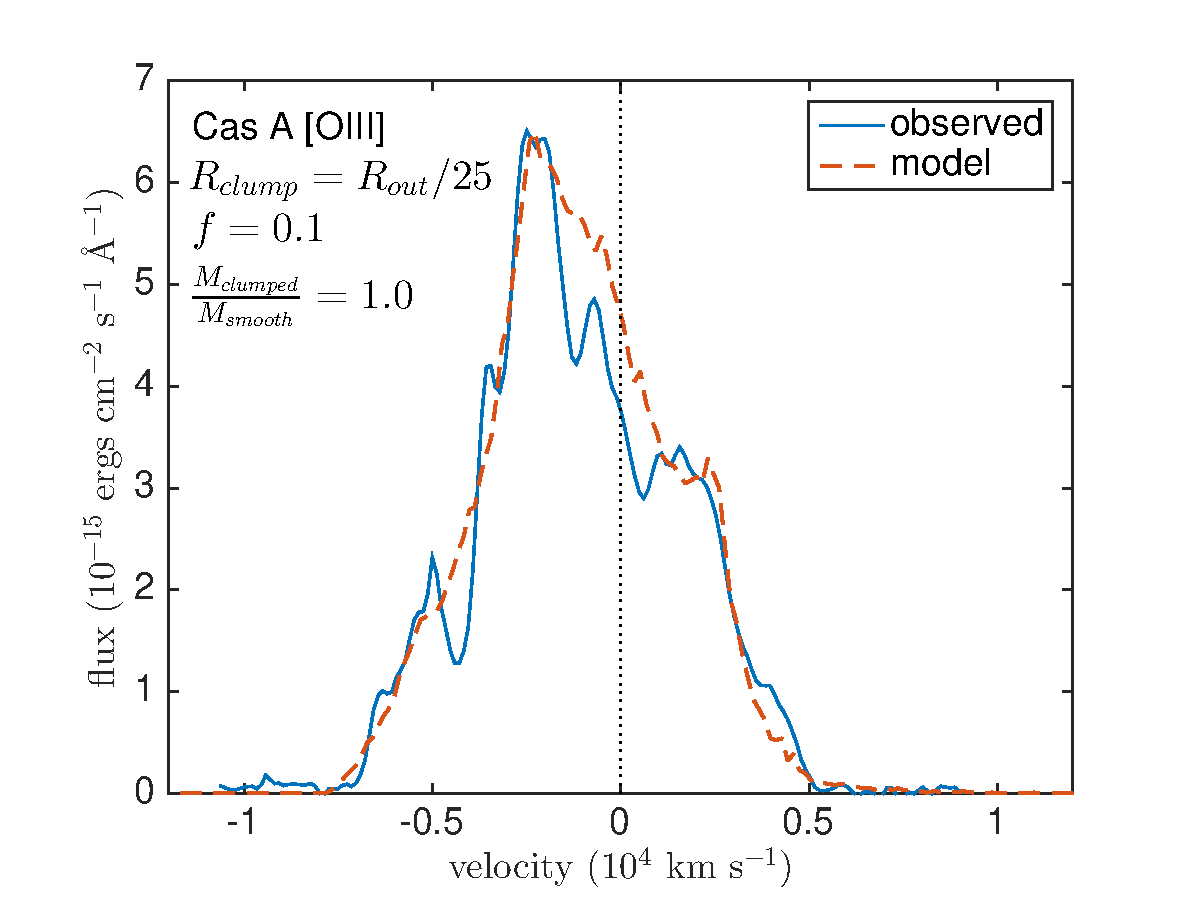
\includegraphics[scale=0.43,clip=true, trim=30 0 40 20]{chapters/chapter6/figs/CasA/clumped/CasA_OIII_c25_f0_1}

\vspace{6mm}
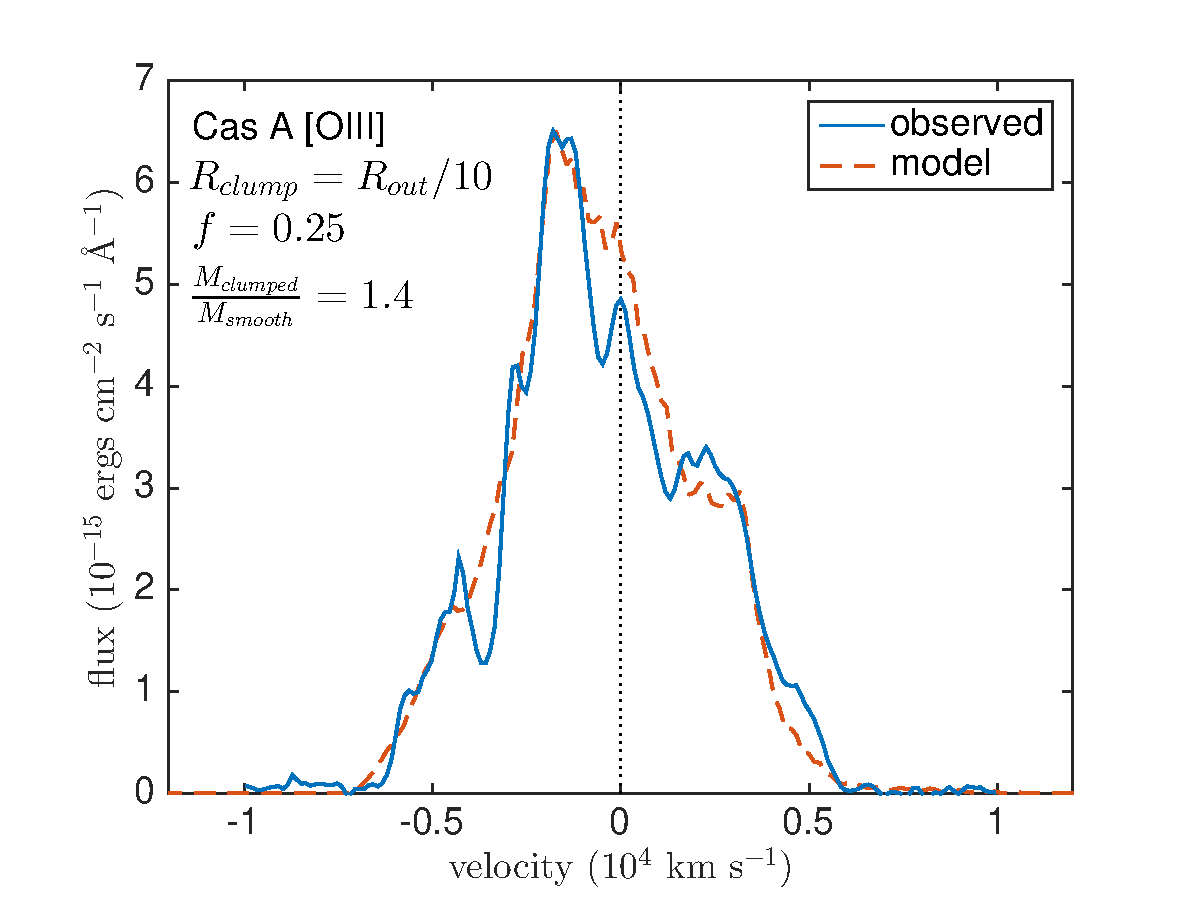
\includegraphics[scale=0.43,clip=true, trim=30 0 50 20]{chapters/chapter6/figs/CasA/clumped/CasA_OIII_c10_f0_25}
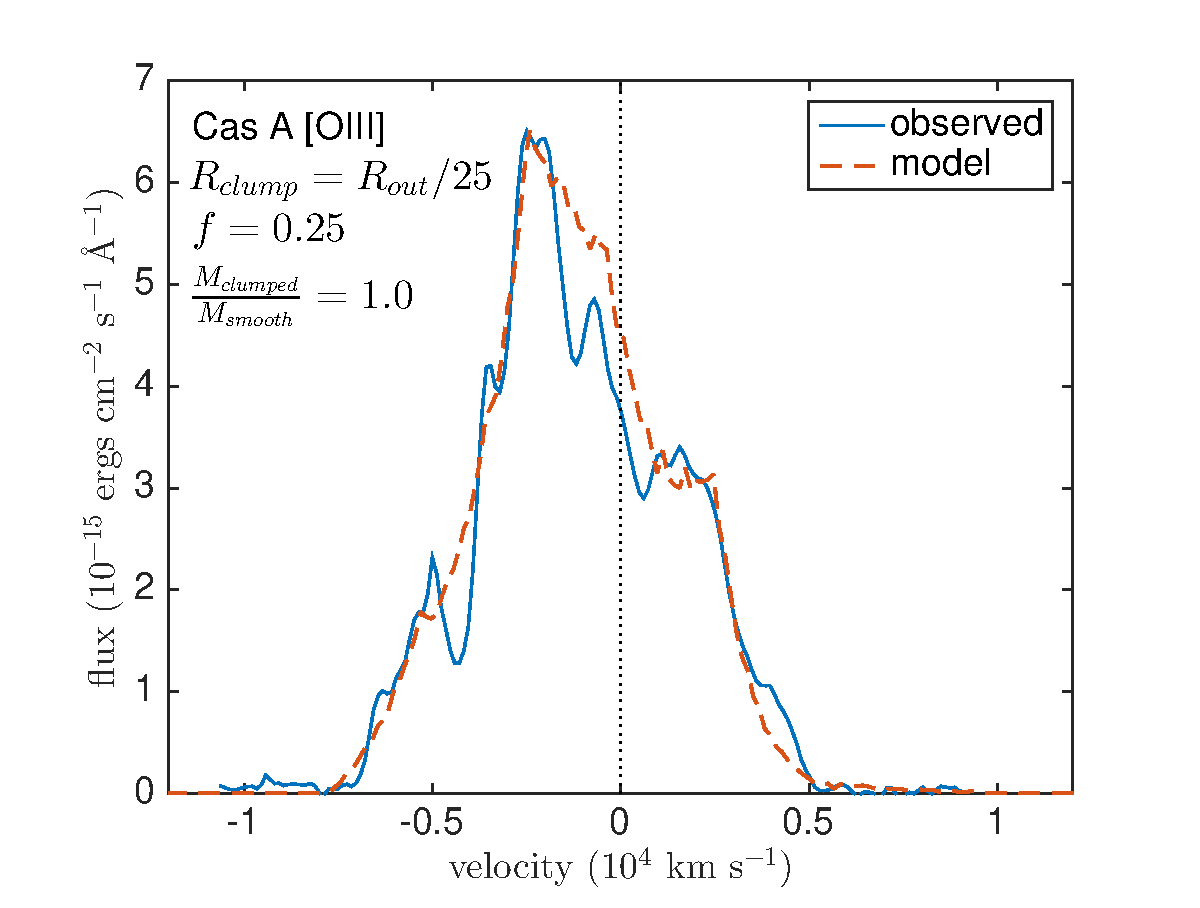
\includegraphics[scale=0.43,clip=true, trim=30 0 40 20]{chapters/chapter6/figs/CasA/clumped/CasA_OIII_c25_f0_25}

\caption{Best clumped dust fits to the Cas~A [O~{\sc iii}]$\lambda\lambda$5007,4959~\AA\ doublet for the parameters described in Tables \ref{CasA_smooth_params} and \ref{CasA_clumped_dust_masses}.  In the left column are fits to the profile using clumps with $R_{clump}=R_{out}/10$ and in the right column are fits using clumps with $R_{clump}=R_{out}/25$.  Each row uses a model that adopts a different clump volume filling factor with $f=0.05$ on the top, $f=0.1$ in the middle and $f=0.25$ on the bottom.  The model profile has been shifted uniformly towards the red by $+700$~km~s$^{-1}$.}
\label{CasA_OIII_clumped}
\end{figure}

The change in the required dust mass is listed in Table \ref{CasA_clumped_dust_masses} as a fraction of the smooth dust mass (e.g. $M_{dust}=1.1$~M$_{\odot}$ for a medium of 50\% astronomical silicates and 50\% amorphous carbon -- see Table \ref{CasA_dust_masses} for other dust masses with different dust compositions).  Whilst clumping serves to increase the required dust mass in all cases, in the most extreme case it is still only by a factor of $\sim$3.5.  The fits for all of these cases are presented in Figure \ref{CasA_OIII_clumped}.

\subsection{Cas~A Discussion}

The models of Cas~A adopt a maximum expansion velocity of $\sim5000$~km~s$^{-1}$ which gives an outer radius of  $5.2\times10^{18}$ cm, equivalent to a diameter of ~3.5~pc.   These values are broadly consistent with an angular diameter of approximately $4'\approx4$~pc at a distance of 3.4~kpc \citep{Reed1995,Hurford1996} and radial velocities between -4000~km~s$^{-1}$ and +6000~km~s$^{-1}$ \citep{DeLaney2010}.  In particular, the need to shift the profiles by -700~km~s$^{-1}$ or -1000~km~s$^{-1}$ in order to fit them is consistent with the expansion velocity asymmetry observed by \citet{DeLaney2010}; an offset of 1000~km~s$^{-1}$ applied to an originally symmetrical distribution between -5000~km~s$^{-1}$ and +5000~km~s$^{-1}$ results exactly in the velocity range that they deduced.  \citet{DeLaney2010} calculate an average velocity offset away from the observer of 859~km~s$^{-1}$, midway between the 700~km~s$^{-1}$ and 1000~km~s$^{-1}$  velocity offsets that I adopt for the [O~{\sc iii}] line and the [O~{\sc i}] and [O~{\sc ii}] lines respectively.  The difference in these values may be a result of different ionisation fractions at different points in the nebula.

\begin{table}
\caption{The fraction of increase in dust mass over the smooth model with parameters as given in Table \ref{CasA_smooth_params} for clumped models with different clump widths and different clump volume filling factors.  The other parameters in the models were fixed at the values given in Table \ref{CasA_smooth_params}.}
\centering
\begin{tabular}{c  c c c}
\hline
clump radius & $f=0.05$ &$f=0.1$&$f=0.25$\\
\hline
$R_{out}/10$ & 3.5 & 1.9 & 1.4 \\
$R_{out}/25$ & 1.6 & 1.0 & 1.0 \\
\hline
\end{tabular}
\label{CasA_clumped_dust_masses}
\end{table}

In general, the structure of the Cas~A remnant is a lot more complex than the simple shell geometry adopted here.  It has been argued that Cas~A is composed of a spherical component, a tilted thick disk, and multiple ejecta jets and optical fast-moving knots all populating the thick disk plane \citep{DeLaney2010}.  These knots  are the cause of some of the noticeable bumpy substructure of the emission lines that I model here.  The models that I have presented above represent a first-order approximation to the geometry of Cas~A and future work will hopefully include a more realistic density distribution.

It is not just the geometrical structure of the Cas~A remnant that is complex.  The chemical composition of the nebula appears also to be extremely varied with evidence for numerous different dust species including silicates, silicon carbide (SiC), alumina (Al$_2$O$_3$) and carbonaceous grains \citep{Rho2008,Arendt2014,Biscaro2014}.  These species also appear to be located in different clumps or regions of the ejecta.  It has even been suggested that the dust could be composed of iron needles which produce a distinctly different SED to more commonly considered grains \citep{Dwek2004}.  Iron grains have a similar absorption efficiency to amorphous carbon grains for a given cross-sectional area but are about three times denser.  Dust masses based on a mixed dust composition of silicate grains and iron grains can therefore be calculated from the dust masses that I have already presented in Table \ref{CasA_dust_masses} by increasing the amorphous carbon dust mass by a factor of $\sim3$.  \citet{Arendt2014} conclude that the entire spectrum of Cas~A can be fitted using only four dust species: Mg$_{0.7}$SiO$_{2.7}$, Mg$_2.4$SiO$_4.4$, Al$_2$O$_3$ and amorphous carbon.  Two of these species (Mg$_{0.7}$SiO$_{2.7}$, Mg$_2.4$SiO$_4.4$) are highly scattering and two (Al$_2$O$_3$ and amorphous carbon) are relatively absorbing.  This  suggests that dust composition models with both silicates and amorphous carbon may be the most representative.  However, whilst there is evidence for a variety of species in the warm dust component, the cool component found by \citet{Barlow2010} that has not yet been heated by the passage of the reverse shock and constitutes the majority of the dust in the ejecta is still of unknown composition \citep{Arendt2014} and so constraining the dust mass is difficult.

Even accounting for the adoption of different species, the dust masses given by my models are generally somewhat higher than the more recent estimates of the dust mass present in Cas A discussed at the start of this section.  However, they are broadly consistent with the estimates by \citet{Dunne2003} of $2-4$~M$_{\odot}$ and by \citet{Dunne2009} of $\sim1$~M$_{\odot}$.  Whilst it seems that there is general agreement over the mass of the warm dust component ($\sim0.1$~M$_{\odot}$), there is still disagreement regarding the mass of cool dust in the ejecta.  This is particularly difficult to establish for Cas~A from photometric observations and SED fitting because of the presence of interstellar clouds of cool dust along the line-of-sight that contribute  the majority of the observed fluxes at sub-mm wavelengths.  Disentangling the relative flux contributions from Cas~A and the interstellar clouds is not straightforward.

Based on SN~1987A, one might expect a cold dust component to be significantly more massive than that of the warm dust component, although these two core-collapse supernovae are of different types. \citet{Biscaro2014} point out that the diffuse nature of Type IIb supernovae compared to their Type IIP counterparts is such that they may struggle to form the molecules and molecular clusters that go on to form dust grains.   

Cas~A is the only object to have had the mass of dust in its ejecta deduced quantitatively using all of the available signatures discussed in Section \ref{three_sigs}.  It is interesting to note that the dust masses inferred from polarised emission and from line profile asymmetries are in broad agreement but are not in agreement with the masses inferred to date from observations in the IR and sub-mm.  Further line profile models of Cas~A that adopt a more realistic and complex geometry  and also include a more representative selection of species will hopefully help to constrain the total dust masses more effectively.  

\section{Conclusions}

It is notable that of the fairly small sample of CCSNe obtained by \citet{Milisavljevic2012} that were still visible spectroscopically at late times, a large number exhibited blue-shifted line profiles.  This feature of the optical spectra of CCSNe at late times is most simply explained by the presence of dust in the ejecta.  I have modelled oxygen and hydrogen lines in the optical region of the spectra of three SNRs and have found that in the majority of cases, even for remnant ages up to 330 years, I can reproduce the  observed line profiles fairly well even with relatively simple models.  Further modelling that allows for more complex geometries may allow even better fits to be obtained.  Regardless, it seems clear that the presence of newly-formed dust in the ejecta of these objects can account for the frequently seen blue-shifting of their line profiles.

\begin{figure}[!t]
\centering
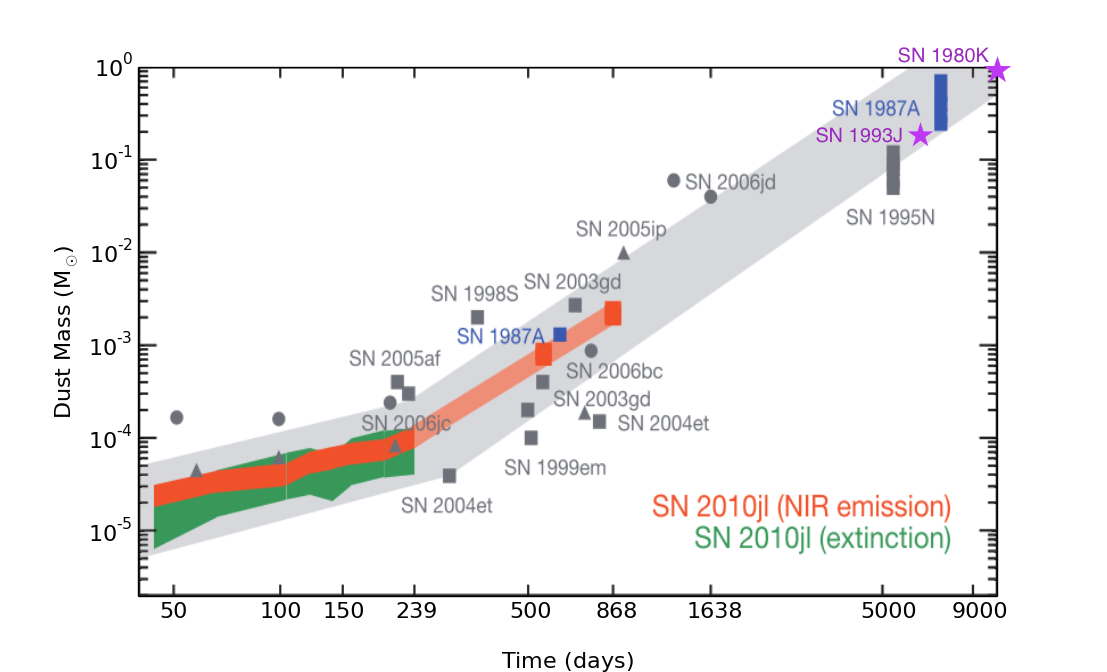
\includegraphics[scale=0.6,clip=true, trim=30 0 50 0]{chapters/chapter6/figs/test2.png}
\caption{Dust formation rates in CCSNe as taken from the study of SN~2010jl by \citet{Gall2014}.  Over-plotted as purple stars are the dust masses derived from the amorphous carbon model for the [O~{\sc i}] doublet for SN~1980K and the silicate model for the [O~{\sc iii}] doublet for SN~1993J showing the excellent agreement between their predicted band and my results.}
\label{dust_masses_gall}
\end{figure}


My aim throughout the modelling of these three objects has been to determine the feasibility that it is dust causing the asymmetry observed in optical line profiles from CCSNe.  It has also been to  determine the dust masses that cause these characteristic dust-affected line profiles.  Whilst the derived dust masses are highly dependent on clumping structures and dust composition, I find that large masses of dust ($0.1-1.0$~M$_{\odot}$) are generally required to account for the degree of blue-shifting observed at late times.  

In particular, I consider the dust formation rates for a number of  CCSNe plotted by \citet{Gall2014}.  They brought together a number of dust mass estimates from the literature for a number of SNe based largely on SED fitting, predominantly at earlier epochs, and extrapolated a dust formation rate.  I present this plot in Figure \ref{dust_masses_gall} and superimpose on it the dust masses that I derived for SN~1980K and SN~1993J.  In both cases, I adopt the dust mass from the more realistic clumped models.  For the purposes of considering how much dust may be formed in the ejecta of CCSNe, I have plotted the maximum dust mass I derived.  For SN~1980K, this is 0.9~M$_{\odot}$ from the amorphous carbon model for the [O~{\sc i}]$\lambda\lambda$6300,6363~\AA\ doublet and for SN~1993J it is 0.18~M$_{\odot}$ from the silicate model for the [O~{\sc iii}] doublet.  These values are in agreement with the dust formation rate extrapolated by \citet{Gall2014} and I note that even the lower dust mass estimates that I derive are still mostly in reasonable agreement.



Cas~A remains unique in being the only remnant of its age for which we have dust mass estimates from line profile asymmetries.  The dust masses I derive here are high, even for the most conservative case and suggest that dust formation in Type IIb supernovae such as SN~1993J and Cas~A is just as effective as for other Type II SNe such as SN~1987A and SN~1980K.  There are strong similarities between the late-time spectra of SN~1993J and Cas~A \citep{Milisavljevic2012}.  Whilst the dust masses that I obtain for SN~1993J are a little lower than predicted by \citet{Gall2014}, the models for the 15 times older Cas~A might indicate that there is more dust yet to form.

Further modelling of these and other supernovae that exhibit characteristically blue-shifted line profiles will hopefully shed more light on this issue.

